\section{Data Architecture}
\label{sec:data-architecture}
This section describes the proposed entities, relationships, integrity constraints
and storage representations. Sections~\ref{sec:use-cases}--\ref{sec:business-rules}
define behaviour; this model must implement those constraints. Types, indexes and
technology choices remain design proposals where not yet agreed.

The companion field reference is compiled from
\nolinkurl{data-architecture-reference.tex}, using
\nolinkurl{technical/data-architecture/data-dictionary.tex}. It supplies field-level
detail omitted from this summary and must be versioned with it. Any conflict with
the requirements requires an explicit correction or decision, not silent precedence.

\subsection{Conceptual Data Model}
\label{sec:data-conceptual}
The proposed model contains 33 entities/associations, including the new WorkerAvailability access association. The complementary ER views show one
model, with contextual entities in grey and endpoint cardinalities explicitly
labelled. Each delivery may have at most one weighing ticket and one analysis,
both of which may be recorded later. ManagerInvitation and AccessGrant
are included. DocumentTemplate and DocumentRendition support the agreed \identifier{UC-20} and
signed worker-specific PDF output. Authentication challenges, outbox operations
and recovery ledgers are technical persistence, not additional business actors.

\subsubsection{Accounts and Business Access}
User is the application identity with a separate administrator/standard system role;
Worker is a business-specific person with no
required login. Workspace separates one owner's properties, campaigns and records.
WorkspaceMembership carries the contextual Owner/Manager role; each active
workspace has one Owner and an account owns at most one workspace.
ManagerInvitation records recipient and reviewed initial grants; acceptance requires
the intended verified account. AccessGrant records actual operations and scope,
including the mandatory insurance constraint. Revocation preserves author/initiator
references. Email verification challenges do not change the User id or ownership.
Workspace stores its business timezone. AccessGrant is keyed by membership,
operation and required property; scopes include parcels and current/future campaigns.
WorkerAvailability links explicitly available workers to manager membership before
scoped work exists; other relevant workers follow authorised scoped records.
It confers no other-property work visibility. Business closure and ownership
transfer are excluded. Account/data erasure requests require the separate privacy
procedure under \decisionref{Q-AA-07}; the model introduces no closure workflow.
Figure~\ref{fig:er-access} summarises the access relationships.

\begin{figure}[!htbp]\centering
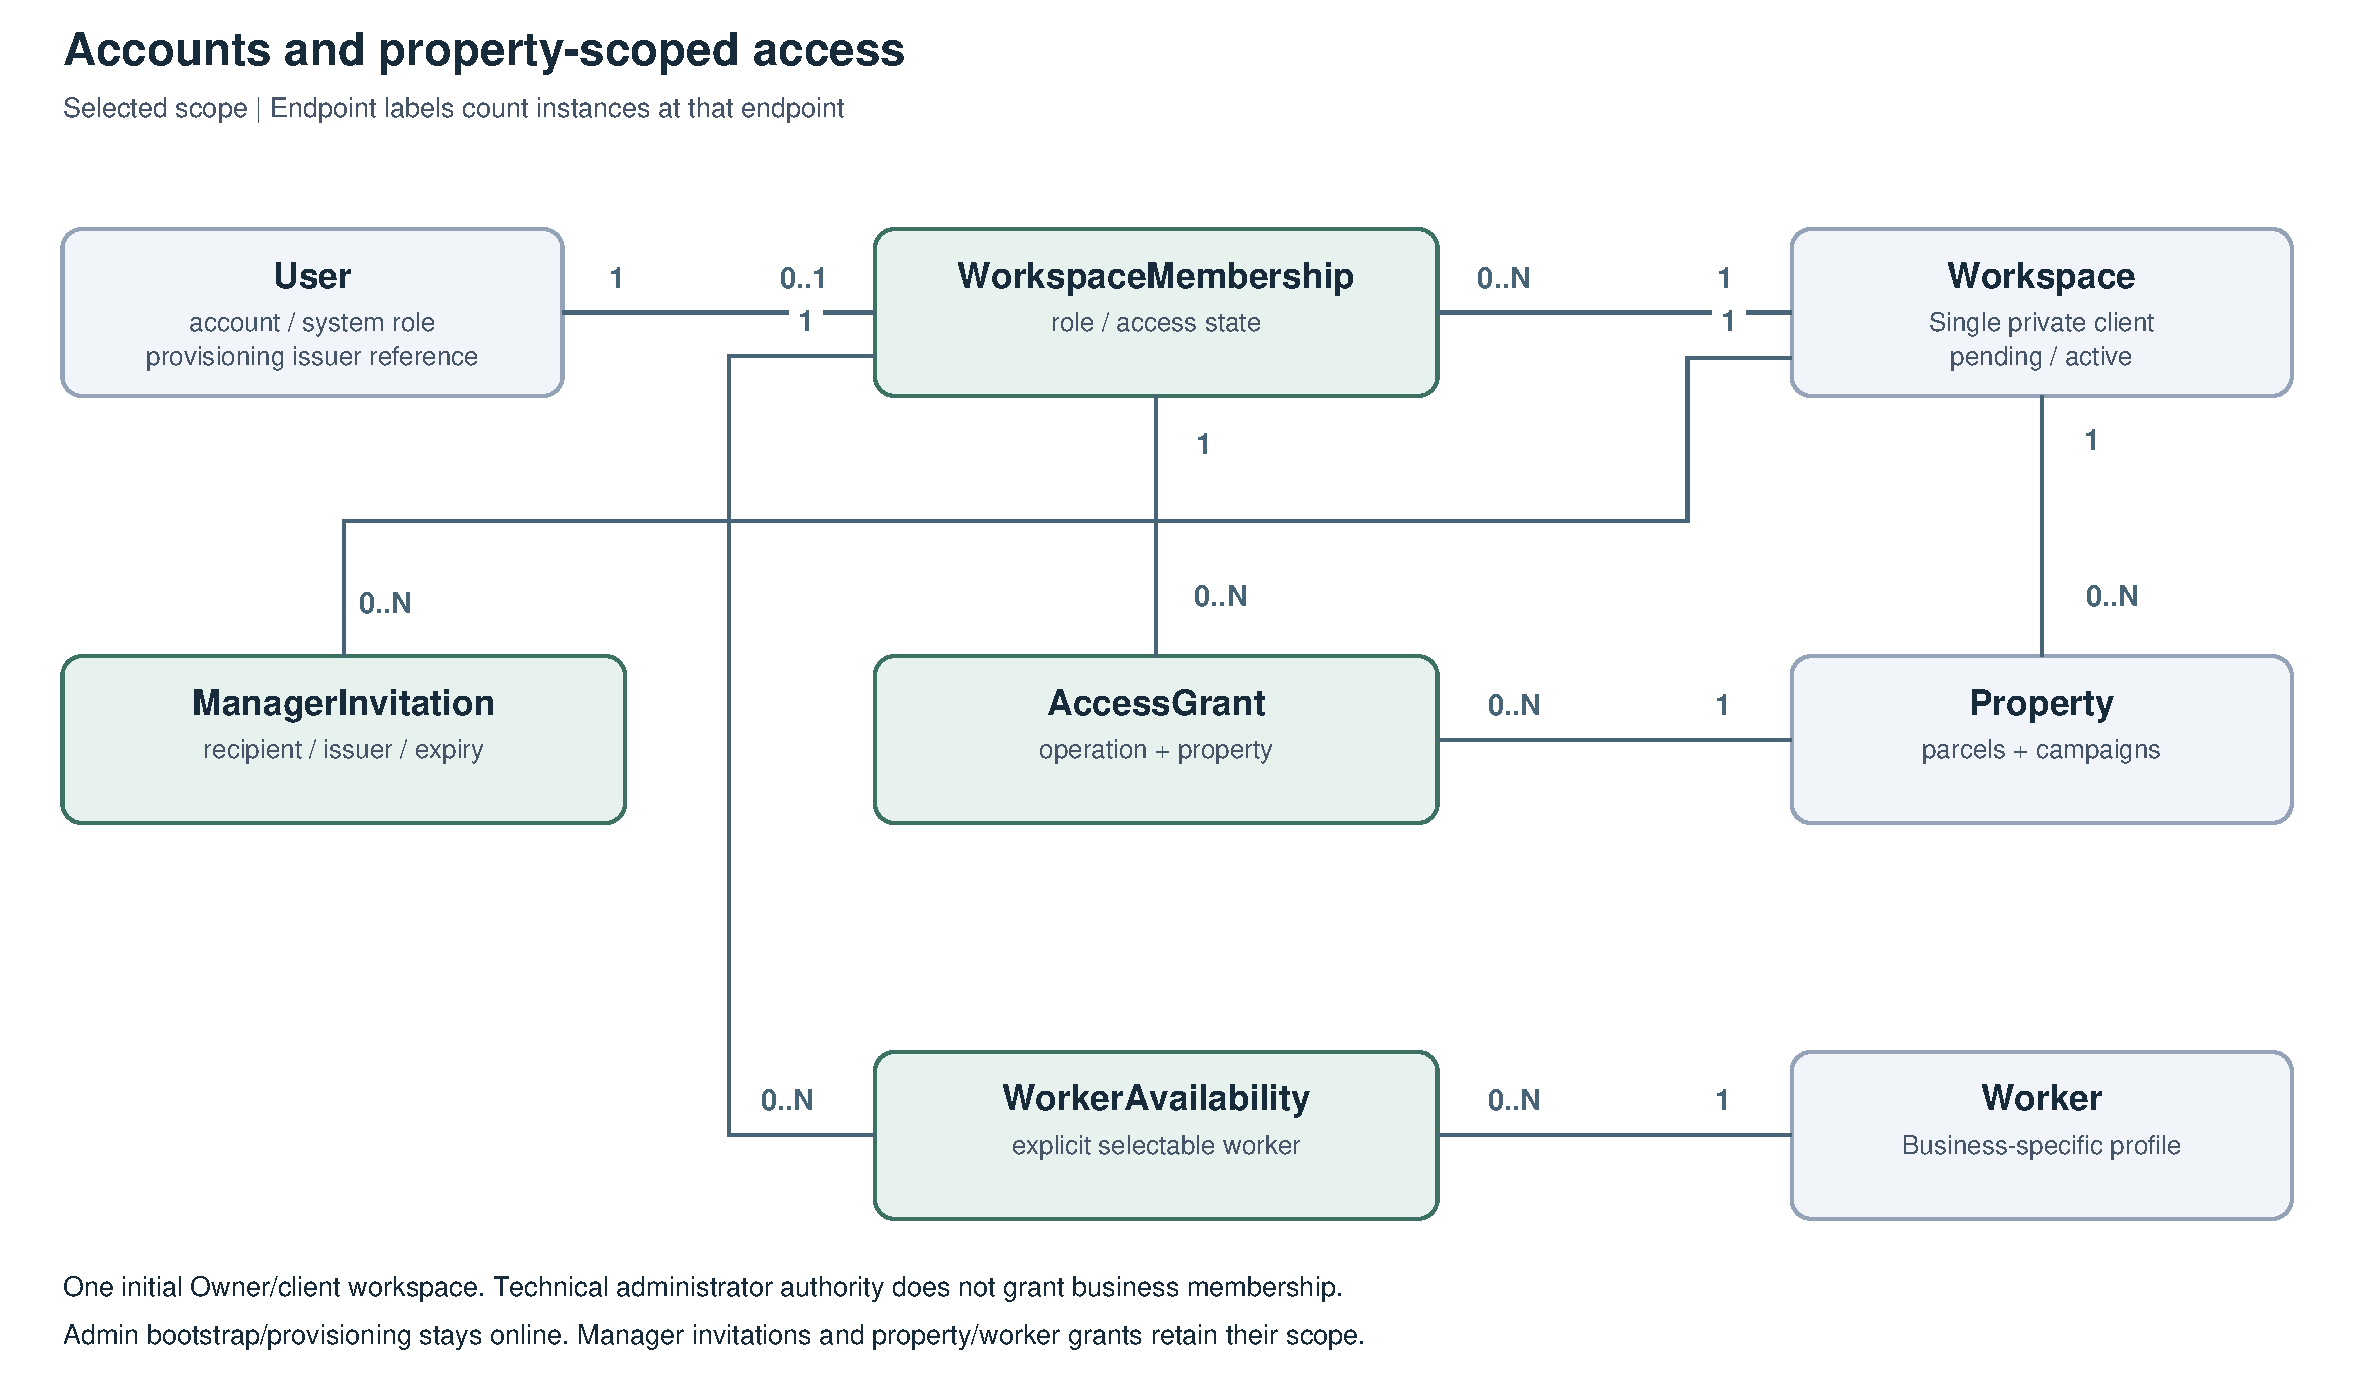
\includegraphics[width=\linewidth]{er-access.pdf}
\caption{Included account, membership, invitation and owner-configured access relationships.}
\label{fig:er-access}
\end{figure}

\paragraph{Provisioning.}
The administrator system role enables initial owner and workspace setup and activation
support only. Owner/Manager remain the operational membership roles. Bootstrap the
first administrator through deployment configuration, with no public administrator
signup. A nullable administrator reference on the provisioned owner records who
initiated setup. The owner workspace and membership remain pending until verified
activation; manager memberships still arise through accepted owner invitations.
The single-client deployment guard prevents a second initial owner/workspace.

\subsubsection{Properties, Parcels and Campaign Coverage}
\label{sec:conceptual-properties}
Property and HarvestCampaign belong independently to a Workspace. Parcel is an
optional reusable division of a Property. CampaignCoverage links a campaign to
one or more whole properties or selected parcels, allowing a campaign to span
several properties without duplicating their records.
Figure~\ref{fig:er-properties-campaigns} shows the coverage relationships.

\begin{figure}[!htbp]
\centering
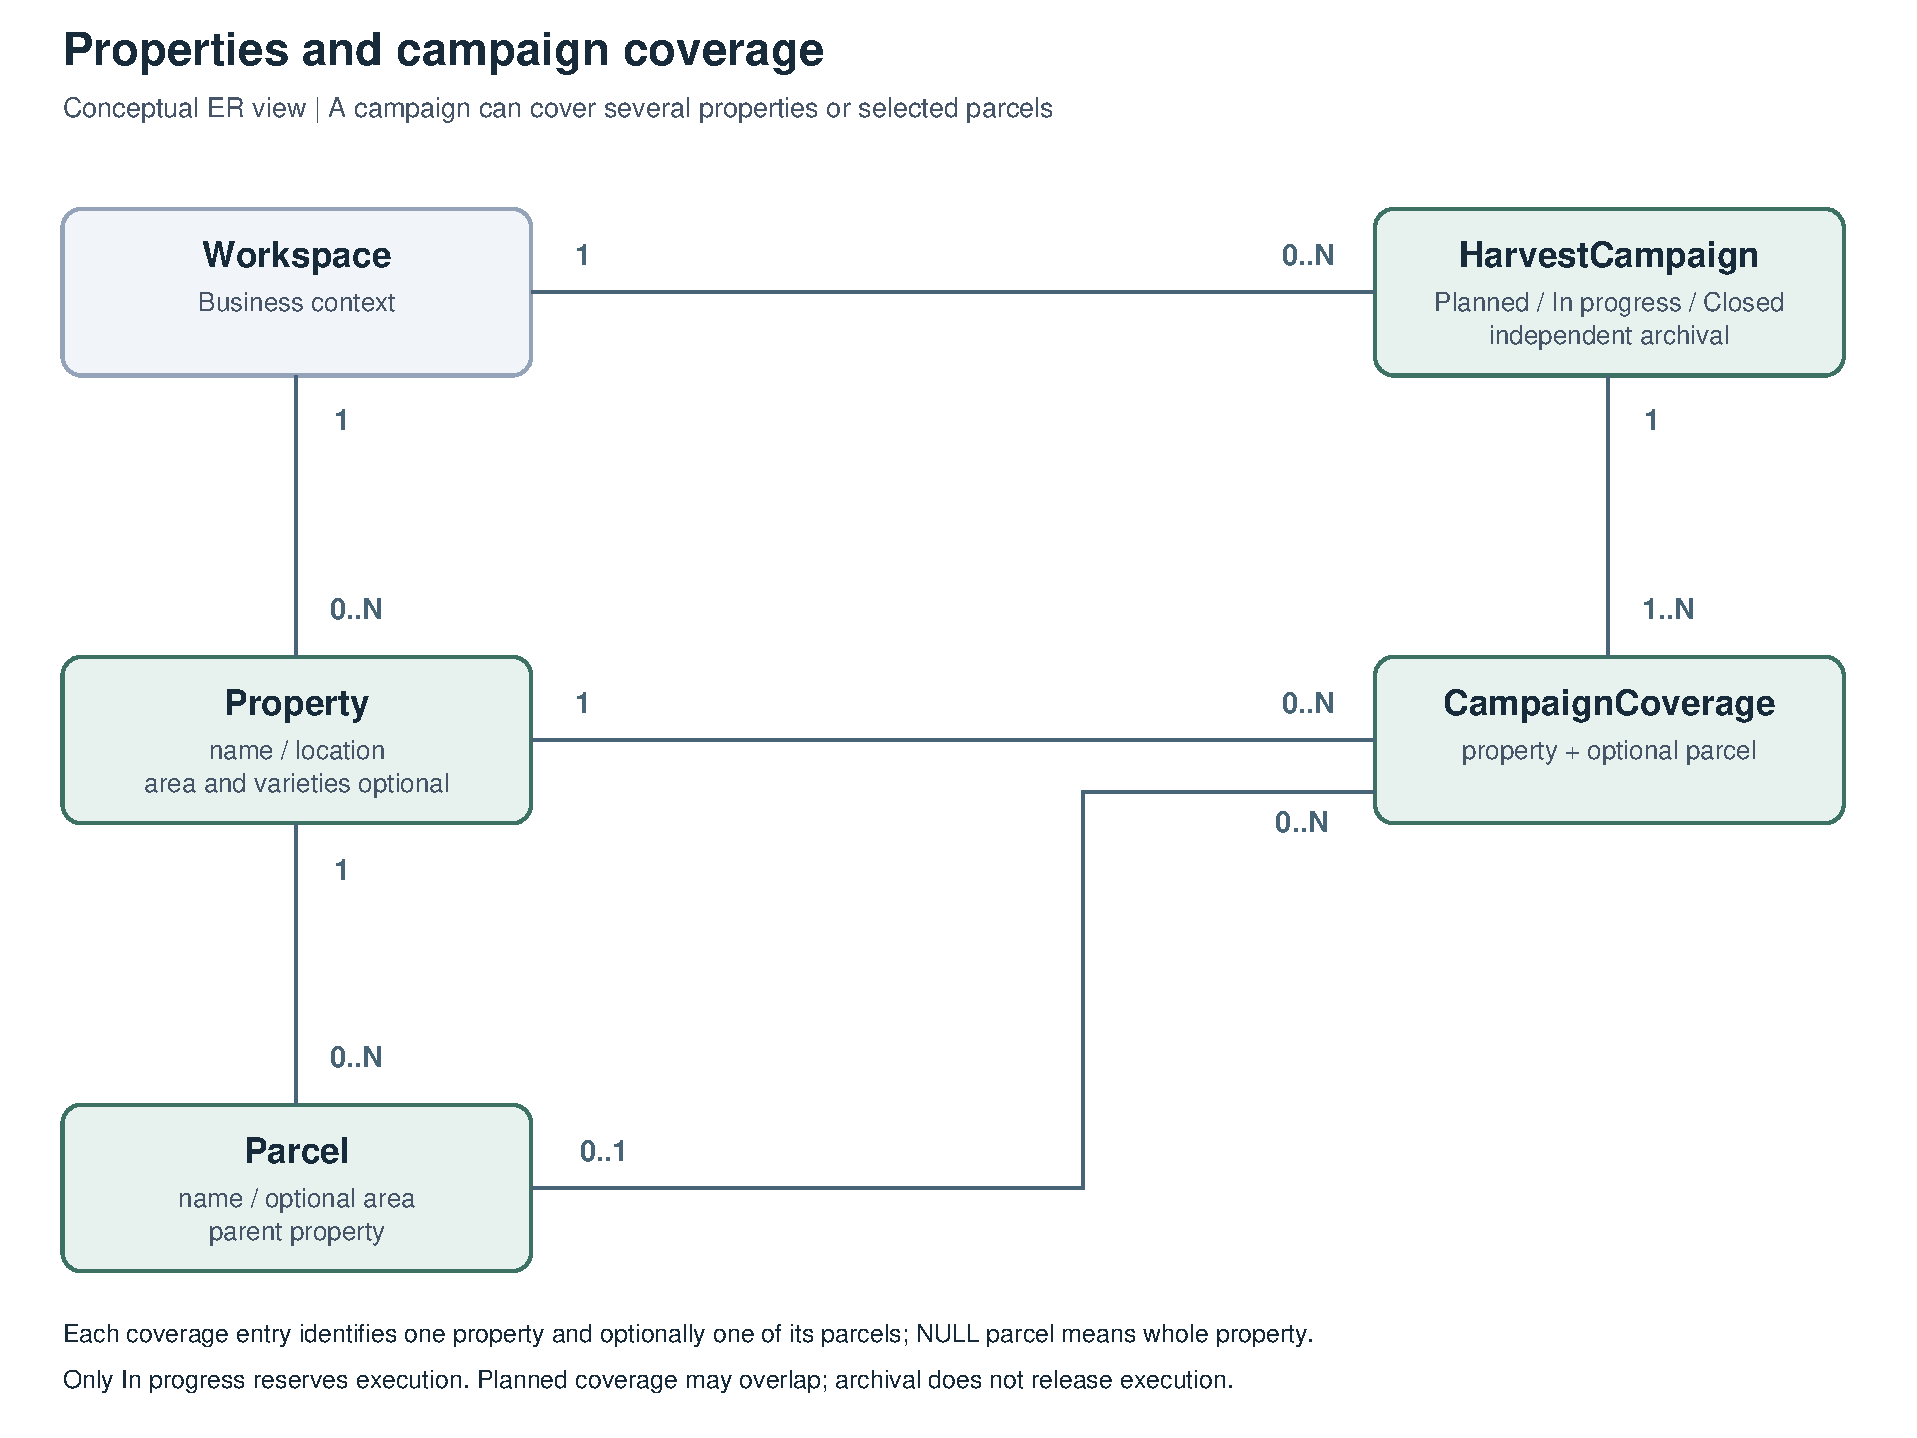
\includegraphics[width=\textwidth]{figures/er-properties-campaigns.pdf}
\caption{Properties, optional parcels and campaign coverage. A coverage entry always identifies a property and optionally one of its parcels.}
\label{fig:er-properties-campaigns}
\end{figure}

A coverage entry always identifies a property and optionally one of its parcels;
an absent parcel denotes whole-property coverage. Operational area references use
the same representation. This preserves the difference between property-level
and parcel-level information when divisions are added later.

HarvestCampaign stores planned start, actual start and actual end separately.
Lifecycle and archival are separate fields because execution/closure govern dates,
while archival controls normal-list visibility. CampaignCoverage is the set against
which start/reopening and In progress coverage changes enforce
\hyperref[br:008]{\identifier{BR-008}}. This cross-record constraint needs transactional
validation; the ER relation alone cannot enforce exclusive execution.

\subsubsection{Business Worker Records}
\label{sec:conceptual-workers}
Worker belongs to a Workspace and retains a stable internal UUID across planning,
attendance, work, driving, document associations and signatures. Mandatory fields
are full name, telephone, official identification type, issuing country and number;
keep the number as text, separately from the UUID and from optional fiscal data.
The type/country/number tuple supports non-unique same-business duplicate lookup;
it is neither a primary key nor a global uniqueness constraint. Identification types are DNI, NIE and Other; Other requires a description. The issuing country is recorded, while country-specific document-format validation is excluded under \decisionref{Q-ID-01}. Offline proposals and their
dependants retain the same UUID through acceptance, as described in
Section~\ref{sec:offline-sync}. Profile updates preserve identity and links;
machinery capability is stored separately from actual tasks.

The profile's activity history queries DailyAttendance, ActualWorkAssignment,
WorkPeriod and WorkBreak under the same worker identity and authorised scope.
Daily and selected-period totals are derived under \identifier{FR-023(c)}; no
additional worker-hours table or copied profile total is required. Corrections
refresh the view from current work records.

\subsubsection{Work Planning, Attendance and Actual Work}
\label{sec:conceptual-workforce}
The model separates expectations, daily presence and actual campaign participation.
WorkPlan groups one campaign's assignments for a working date. PlannedAssignment
identifies a worker and area, with optional PlannedWorkPeriod and PlannedBreak
records. These tables retain the proposal independently of subsequent actual work.
Figures~\ref{fig:er-planning} and~\ref{fig:er-actual-work} show planning and actual work,
respectively.

\begin{figure}[!htbp]
    \centering
    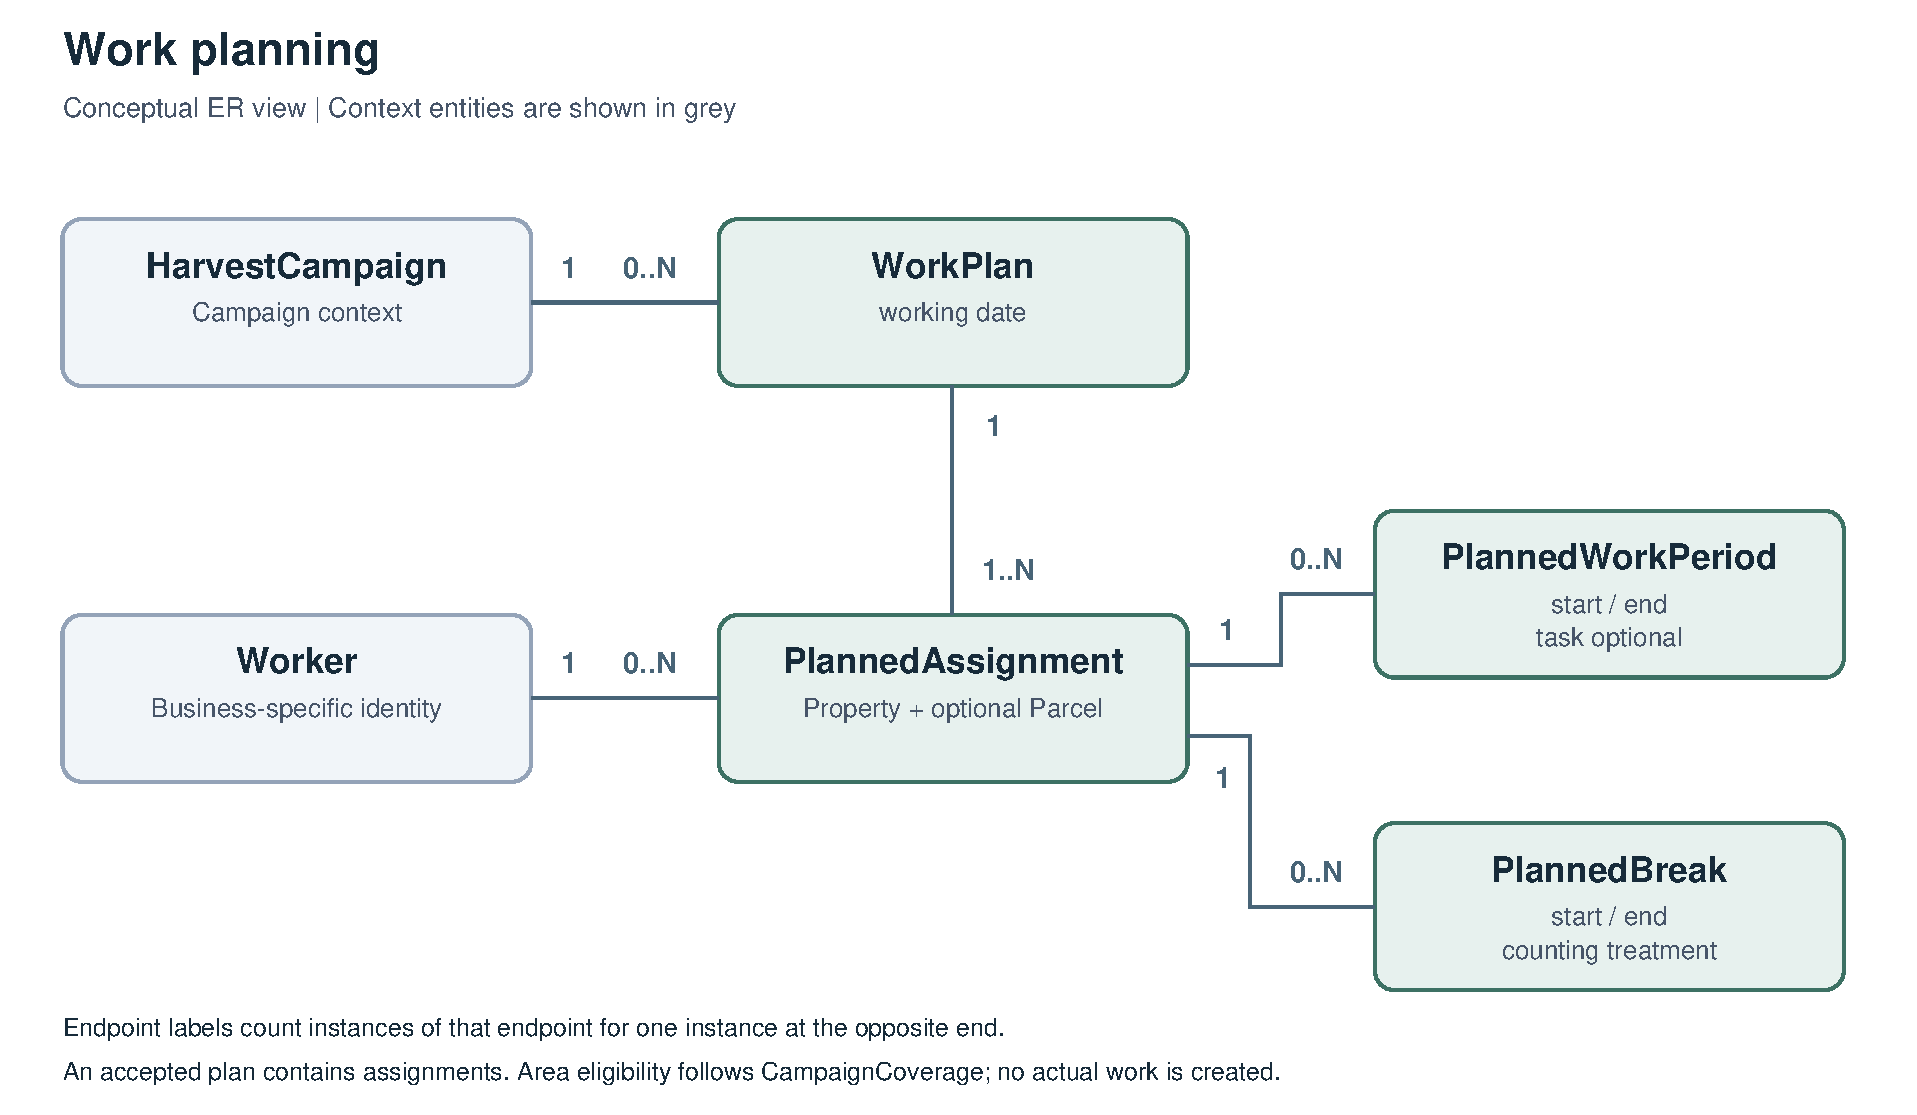
\includegraphics[width=\textwidth]{figures/er-planning.pdf}
    \caption{Conceptual relationships for work planning.
    Context entities are shown in grey; area references are summarised.}
    \label{fig:er-planning}
\end{figure}

\paragraph{Daily presence and campaign participation.}
DailyAttendance identifies one worker and working date within a workspace, without
a campaign reference. ActualWorkAssignment supplies the campaign and area context.
This supports one daily attendance decision across several campaigns and records
participation before hours or tasks are complete. An actual assignment may refer
to a source PlannedAssignment, but no mandatory one-to-one correspondence is imposed.

\begin{figure}[!htbp]
    \centering
    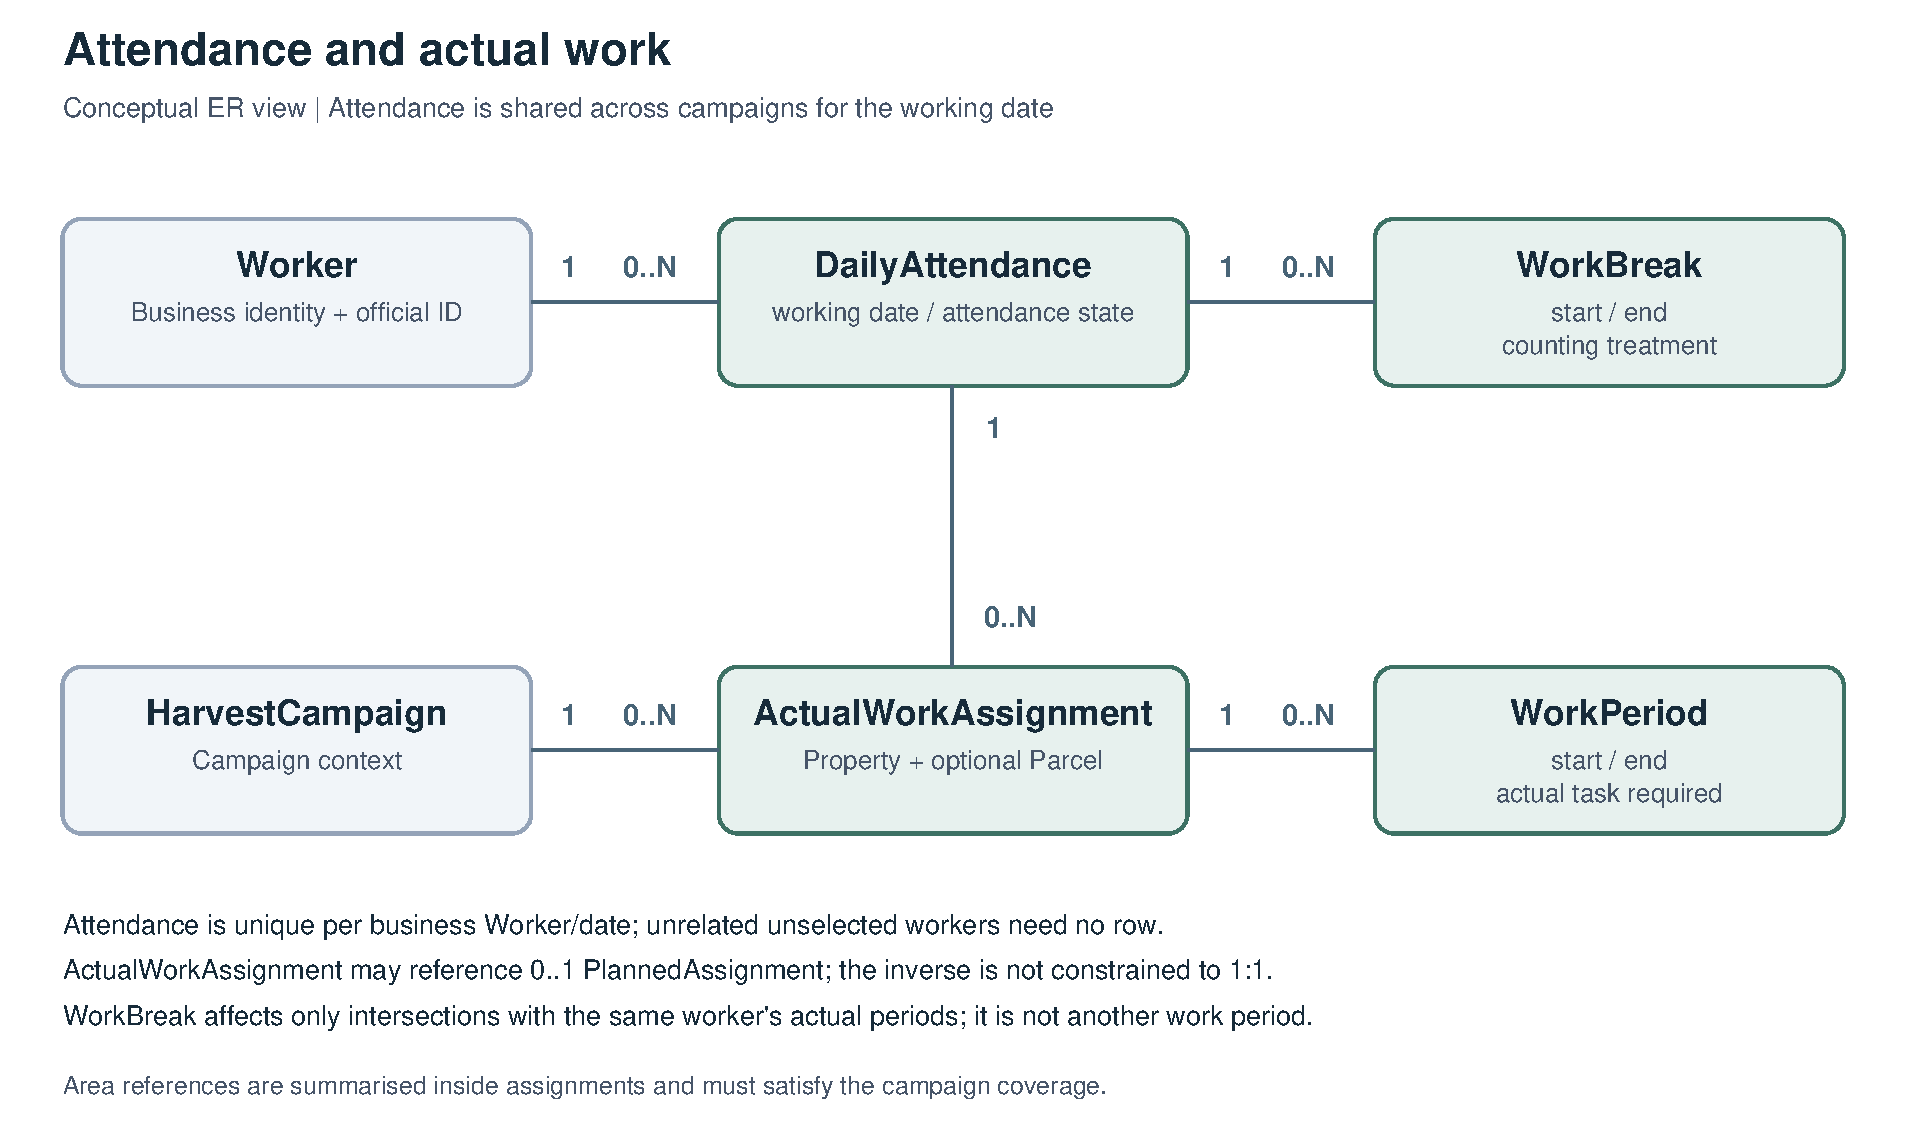
\includegraphics[width=\textwidth]{figures/er-actual-work.pdf}
    \caption{Conceptual relationships for daily attendance and actual work.
    The optional reference to a planned assignment does not impose a one-to-one correspondence.}
    \label{fig:er-actual-work}
\end{figure}

\paragraph{Intervals and breaks.}
WorkPeriod belongs to an actual assignment; WorkBreak belongs to daily attendance.
The latter placement lets a worker's break intersect consecutive task or campaign
periods without duplicating it. Complete start/end timestamps support intervals
crossing midnight and cross-campaign overlap checks. Missing hours are represented
by the absence of complete periods; each confirmed complete period requires
its actual task. An incomplete assignment is not converted into zero hours.

Planning and confirmation conditions are defined in \hyperref[br:017]{\identifier{BR-017}}--\hyperref[br:021]{\identifier{BR-021}};
the counted-time formula is in Section~\ref{sec:counted-working-time}.
Completion and correction use Sections~\ref{sec:completion-correction} and~\ref{sec:work-corrections}, without a separate
entity for every historical field value.

\paragraph{Expected versus unrelated workers.}
DailyAttendance is sparse: it does not require a row for every worker/date. Derive
expectations from selected/planned or actual assignments under
\hyperref[br:018]{\identifier{BR-018}}. This avoids recording non-selection as absence. Pending
records reference locally created Worker UUIDs without creating a second daily
attendance after acceptance.

\subsubsection{Deliveries, Loads and Cooperative Results}
Delivery belongs to one campaign and has one associated TransportRecord, with a
registered Worker driver. OliveBatch stores one actual source property and optional
parcel, with known source quantities separate from official ticket weights.
TransportRecord may retain a transport-document reference and declared origin;
these do not allocate a mixed load or make parcels mandatory.
Figure~\ref{fig:er-deliveries} shows the delivery and source-result relationships.
\begin{figure}[!htbp]\centering
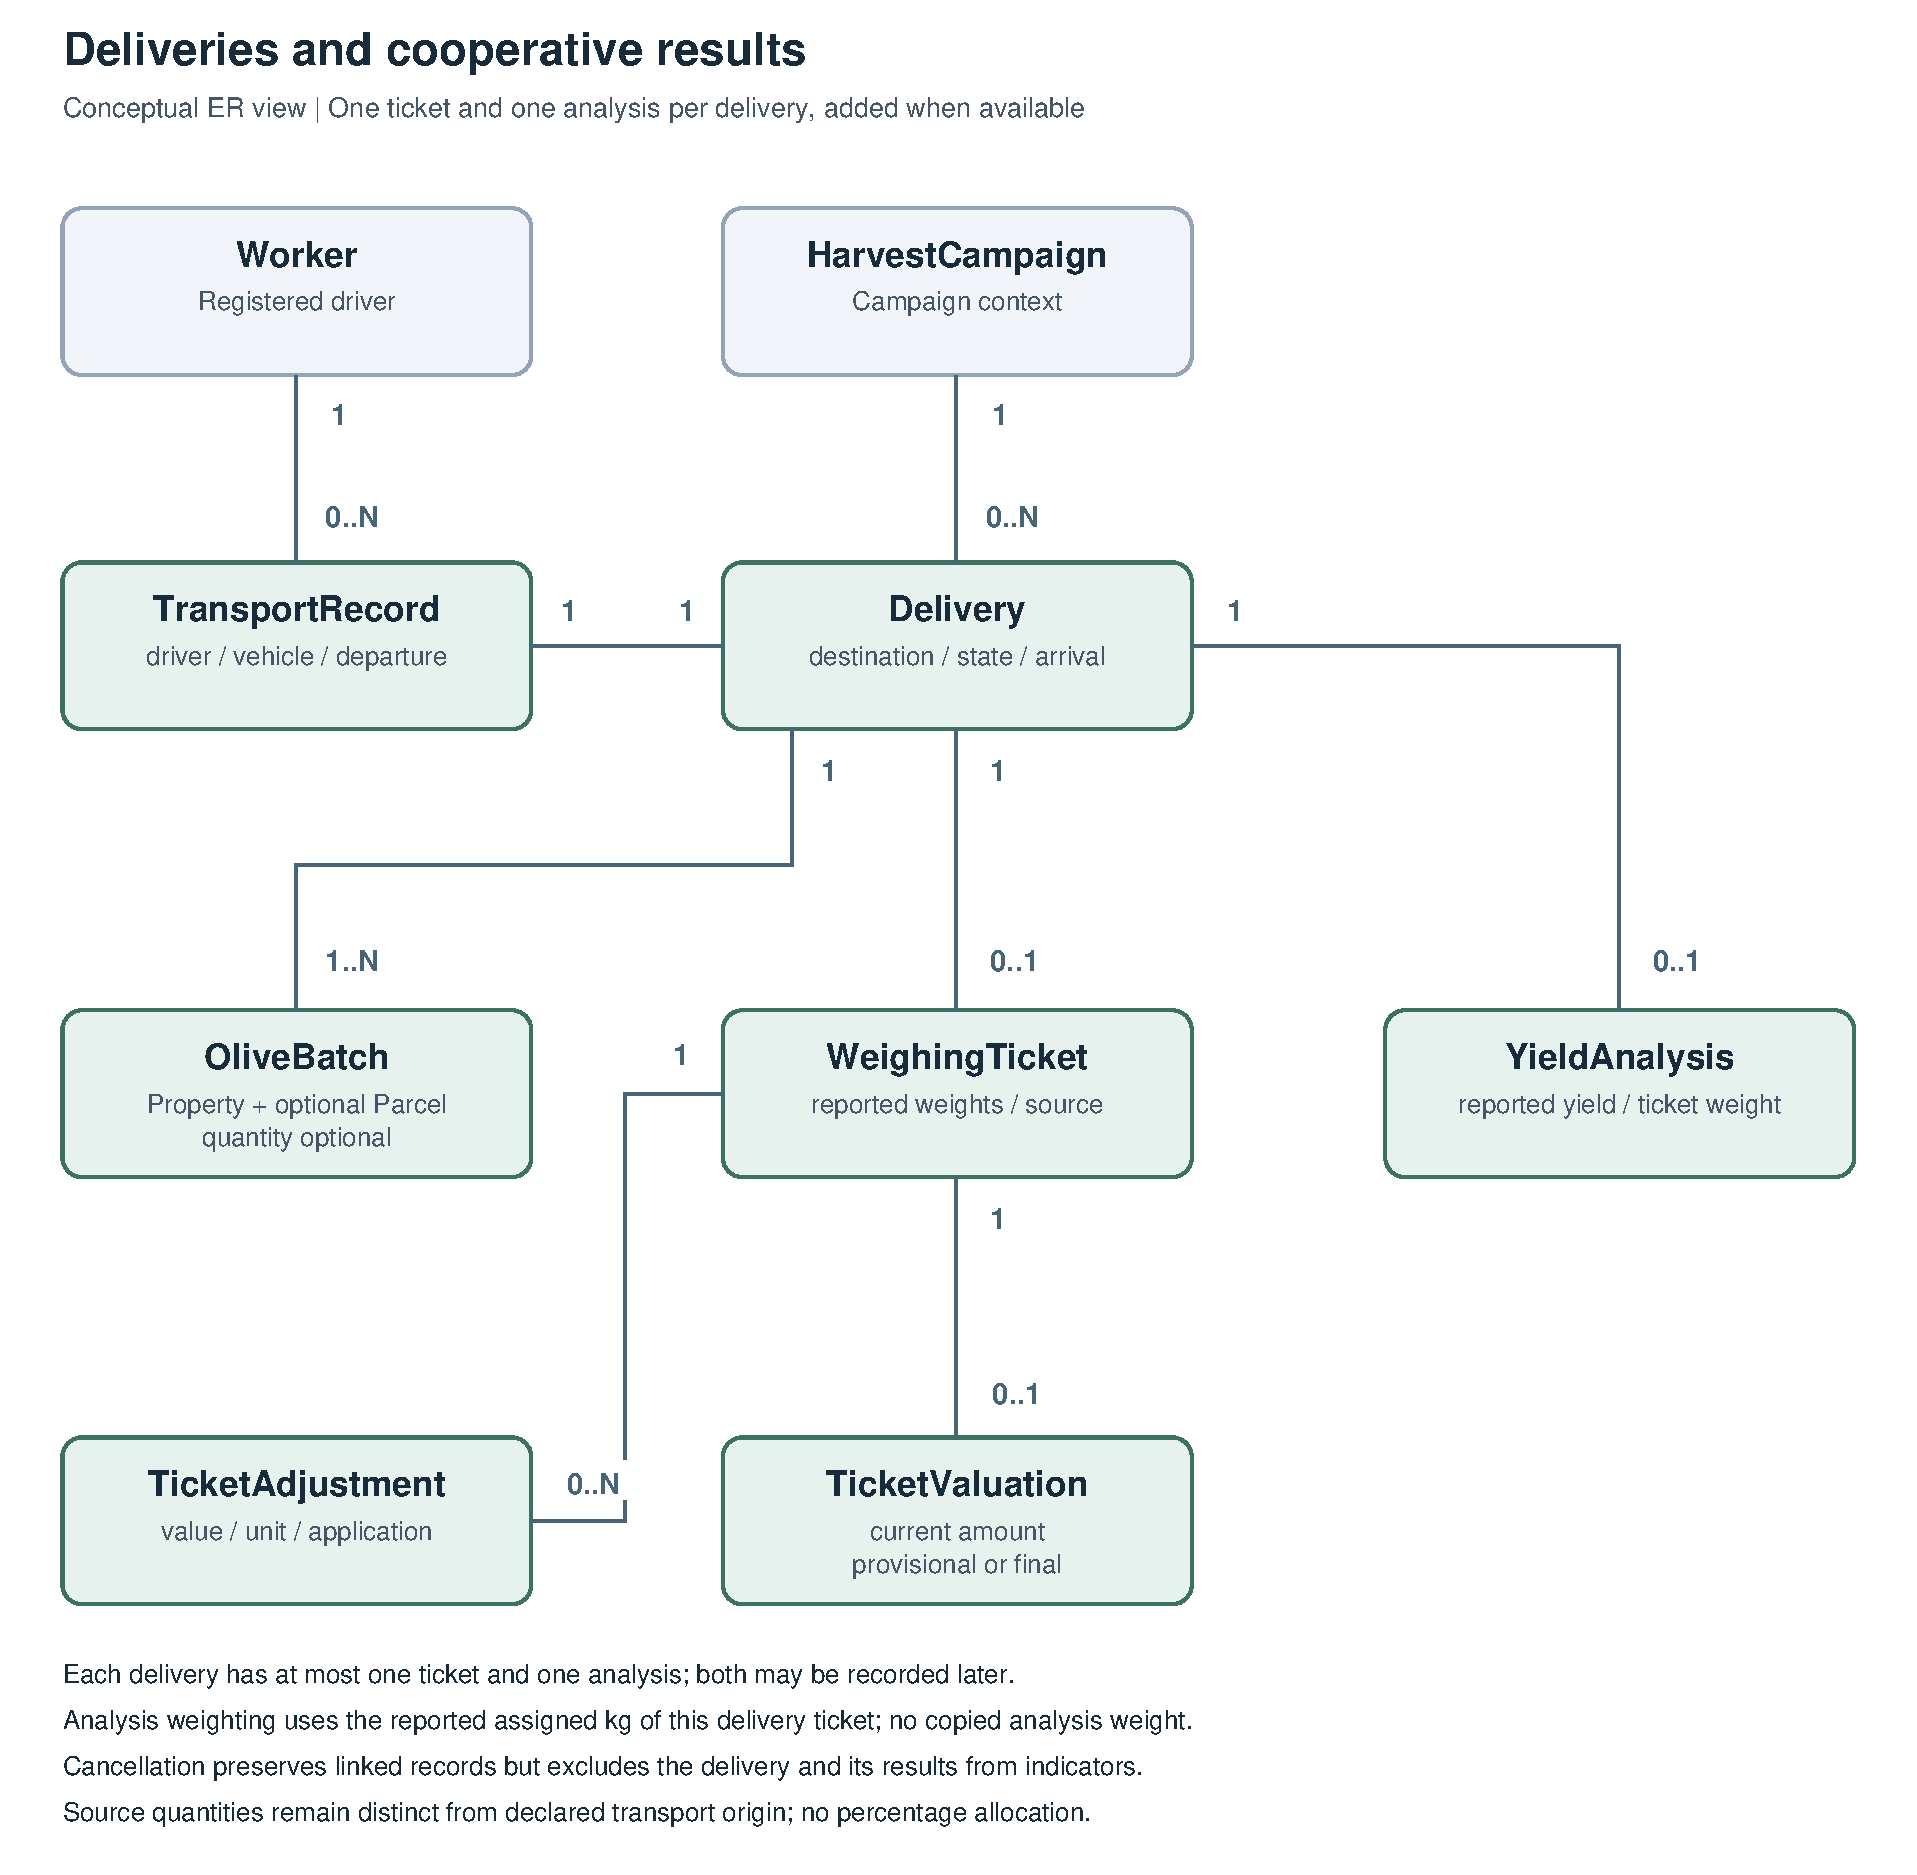
\includegraphics[width=\linewidth]{er-deliveries.pdf}
\caption{Each delivery has at most one ticket and one analysis. Source batches remain distinct from official weights.}
\label{fig:er-deliveries}
\end{figure}
WeighingTicket has a unique delivery reference and an optional canonical reported
accepted assigned weight in kg. Other weights retain source meanings/units. Optional
weighing start/end and reported excess duration are descriptive source facts.
TicketAdjustment also represents reported monetary penalties, protected by financial
grants; the application does not calculate or reapply them.
YieldAnalysis has a unique delivery reference and the reported yield percentage.
Its weighting reference is reached through the delivery's ticket; no independently
editable reference-weight copy is stored. TicketValuation is one current reported
amount per ticket. SourceAttachment supplies separate evidence links.
Source records may exist while Delivery is In transport. Indicator queries use
the Delivered, non-cancelled parent predicate in \hyperref[br:038]{\identifier{BR-038}}; source
existence alone does not confirm receipt.
The current model records known quantities in OliveBatch and one total amount
in TicketValuation; it has no field for monetary amounts by source. Mixed-load
amounts therefore remain unallocated by property/parcel, even when source quantities
are known. Supporting reported source amounts would require an explicit model
extension and review. No monetary allocation proportional to weight is inferred.
Delivery cancellation stores reason, time and actor while preserving dependent
records; lifecycle and correction behaviour follow \hyperref[br:031]{\identifier{BR-031}}.
Eligible hard deletion removes composed TransportRecord and OliveBatch rows in the
same validated operation, only when no ticket, analysis, valuation or evidence blocks it.

\paragraph{Ticket source fields.}
A validated source metadata snapshot holds source date/season, line, sample/member
references, quality/variety, municipality, literal POL/PAR/REC/PARAJE and locator
(Table~\ref{tab:source-ticket}). These source facts do not silently edit properties,
parcels, worker identities or transport records. Total kg and other source weights use validated reported-weight entries; KILOS ASIGNADOS uses only the typed canonical assigned kg field, which remains unknown if no accepted weight was reported. MEDIANERIA records the accepted percentage without generating a second assigned-weight value. Store printed
duration in seconds separately from start/end and excess time, with discrepancies
flagged for review. No penalty-calculation entity or integration is introduced.

\subsubsection{Worker Documents, Generation and Signatures}
Document has one required Worker reference and identifies category/title/subtype;
DocumentVersion holds that worker's accepted source and version-specific metadata.
WorkerSignature binds the document worker to one reviewed version and identifies
the initiating User separately. The worker signs, not the initiating account.
Figure~\ref{fig:er-documents} shows individual document sources and signing results.
\begin{figure}[!htbp]\centering
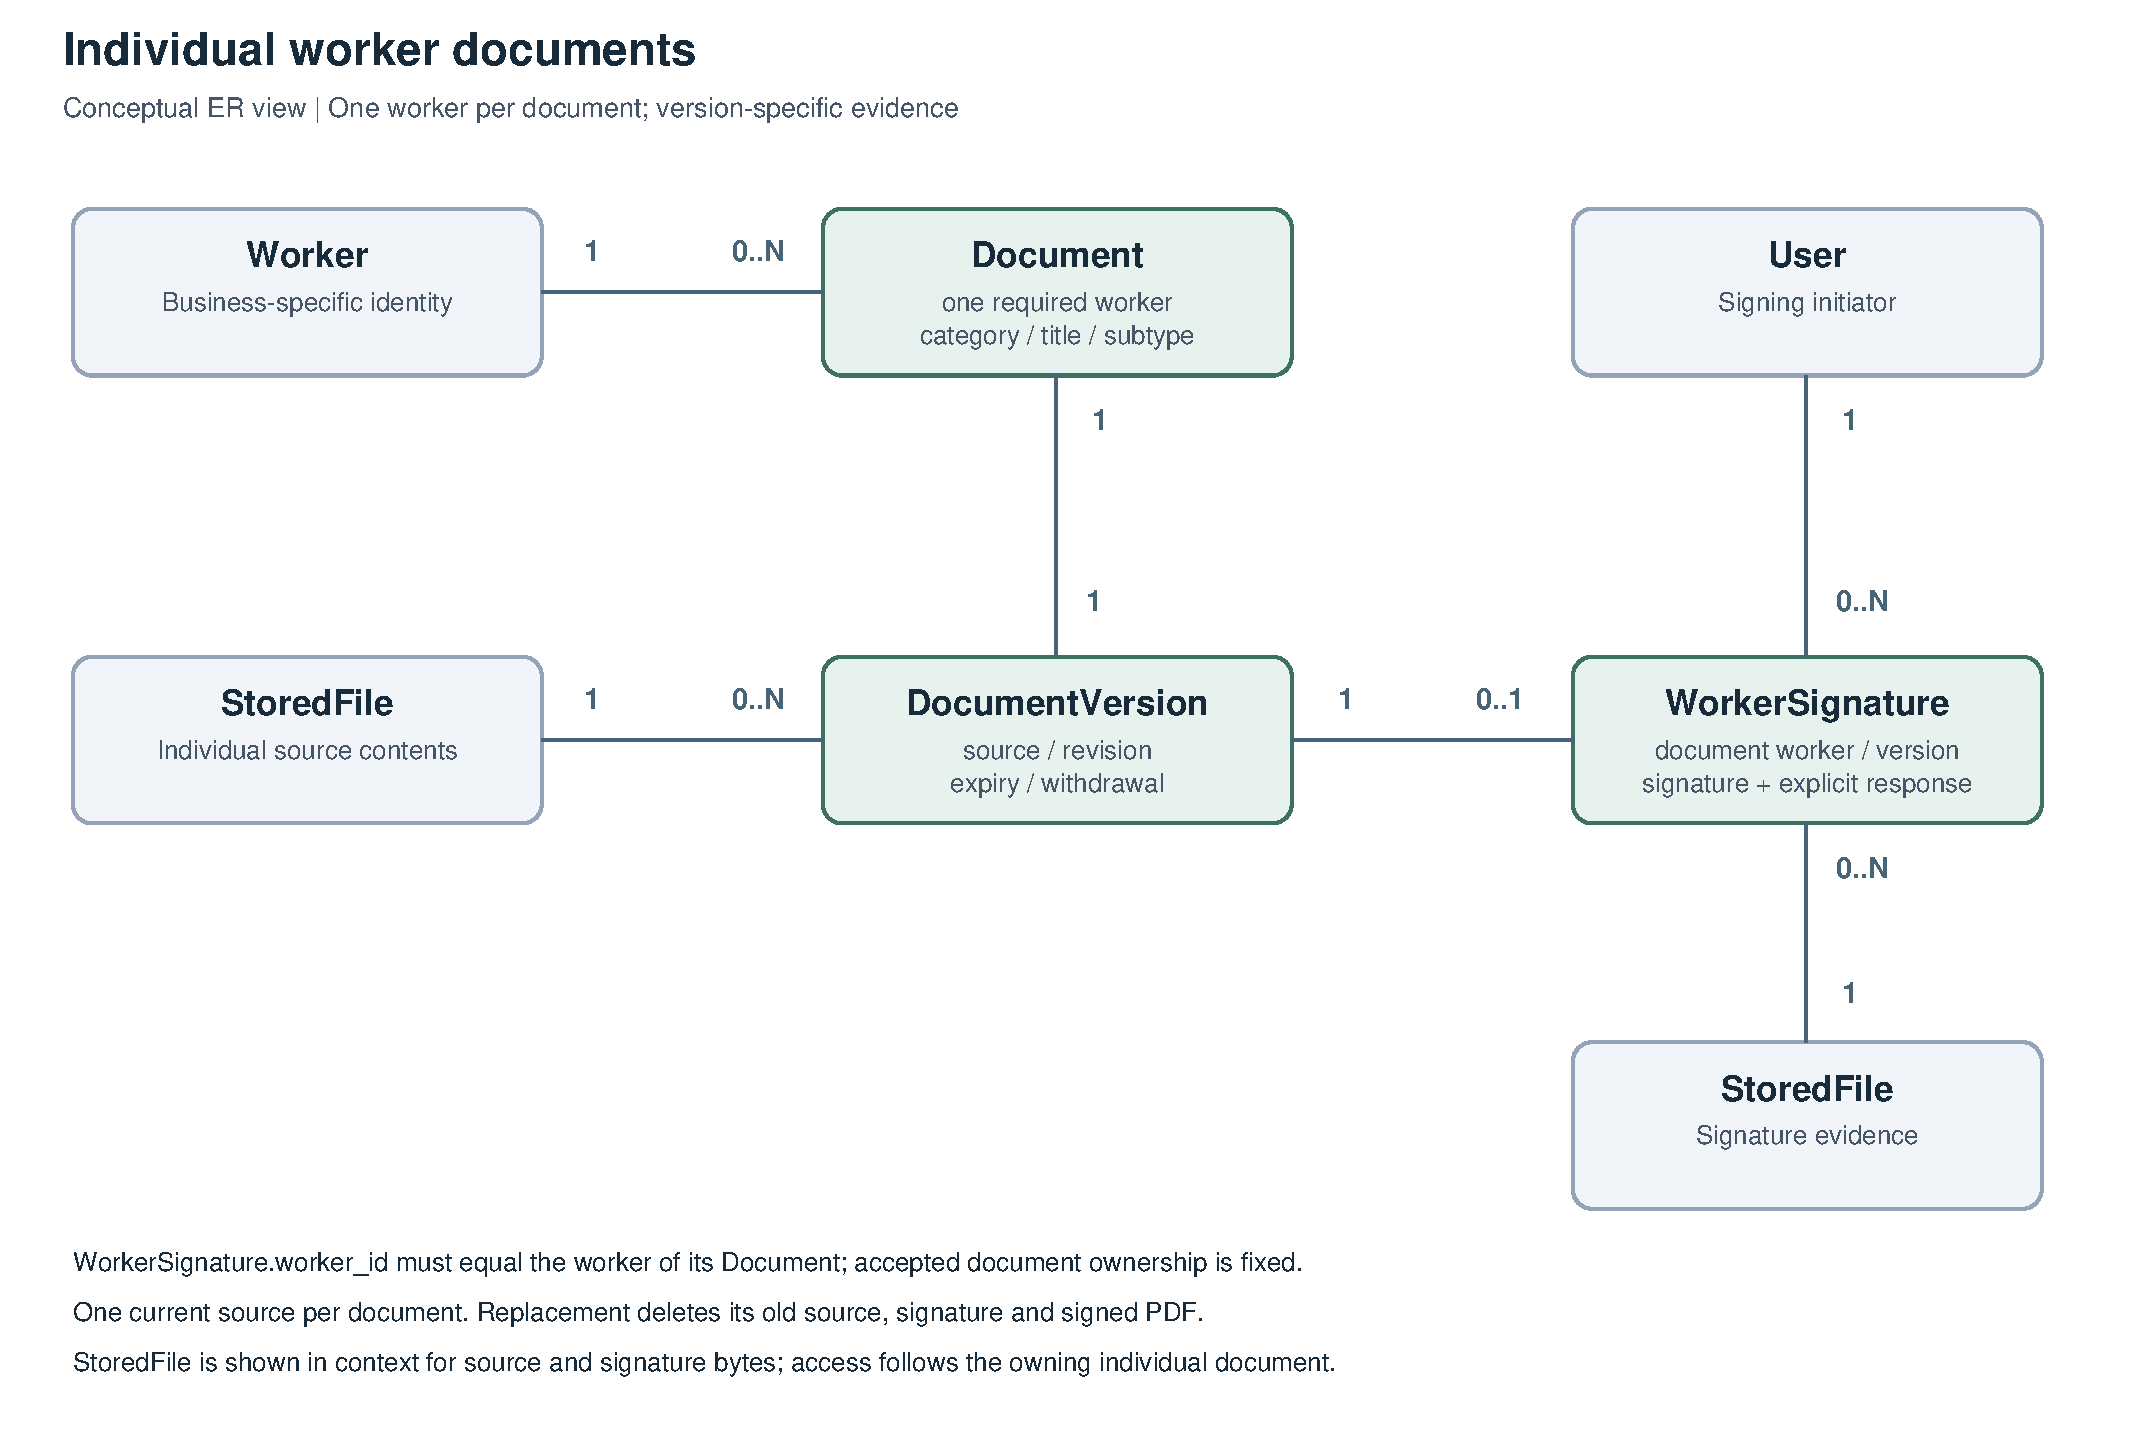
\includegraphics[width=\linewidth]{er-documents.pdf}
\caption{Individual sources and worker/version signing results. StoredFile is one entity shown in contextual views.}
\label{fig:er-documents}
\end{figure}
DocumentVersion separates source identity, currency, withdrawal, recorded expiry
and external-signature declaration. WorkerSignature records individual signing;
retention/cleanup follows \hyperref[br:026]{\identifier{BR-026}}, including deletion of a superseded source, signature and PDF and temporary recovery of ineligible signing proposals under \decisionref{Q-DOC-04}.

DocumentTemplate supplies an available model, category, revision and field schema.
Generated DocumentVersion records the template reference/revision and reviewed
input snapshot. Signing preserves that source and adds worker-specific evidence
and a derived signed PDF under \identifier{FR-042(d)}, for uploaded and generated versions alike.
DocumentRendition links a derived PDF to that version and worker. The worker-specific
rendition contains the document worker's captured signature and explicit response
where required, preserving source contents. Regeneration is not another signing event.
Figure~\ref{fig:er-generation} shows how generation and renditions relate to the source.
\begin{figure}[!htbp]\centering
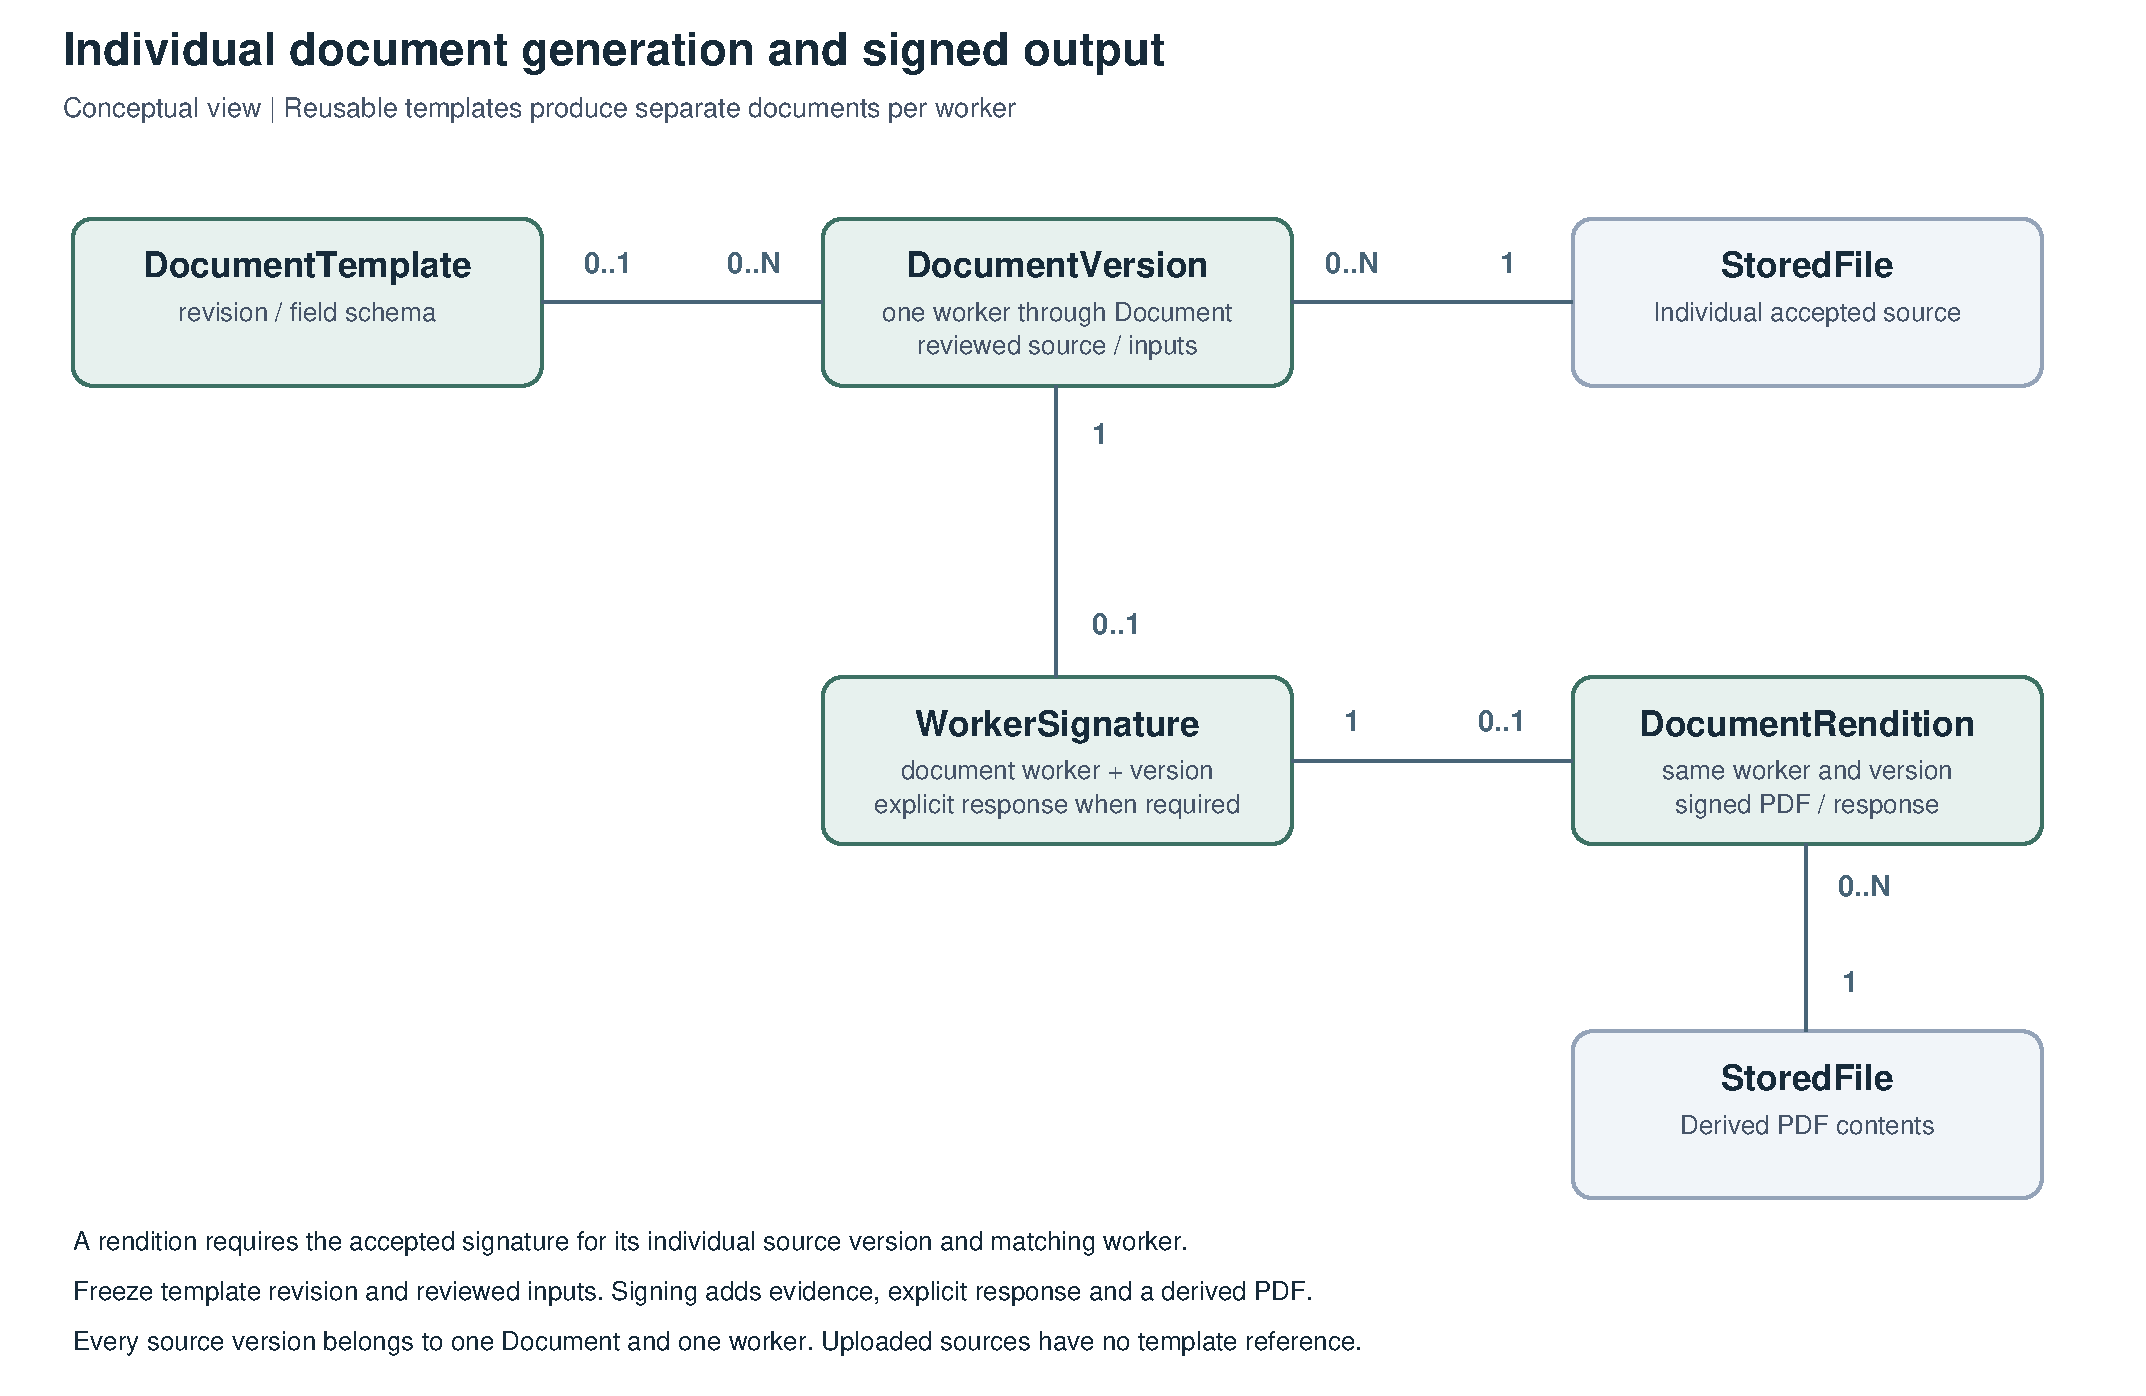
\includegraphics[width=\linewidth]{er-generation.pdf}
\caption{Template-based generation and worker-specific derived signed PDFs. Uploaded versions have no template reference.}
\label{fig:er-generation}
\end{figure}
The supplied inventory appears in Table~\ref{tab:source-forms}; the selected Spanish wording is preserved, with rendering and field mapping to be tested by the team. Document records subtype, DocumentVersion freezes source/template
inputs and any reviewed external response, and WorkerSignature binds an explicit
response to the signing event. Generation leaves consent undecided until signing;
evidence/PDF preserves the decision. Every document has one worker and one current accepted source. Replacement deletes the previous source, signature and PDF without a consultable history. Reusing a
template creates independent documents for each selected worker. Identity/permit originals are uploaded evidence; generation does not issue
them. Worker activity is derived in the profile under \identifier{FR-023}, without a dedicated attendance-document workflow. Source generation/acceptance
requires connectivity, while an accepted prepared version may be signed offline.

\subsubsection{Stored Files and Source Evidence}
\label{sec:conceptual-files}
StoredFile holds storage metadata shared by document contents, captured signatures
and source evidence. SourceAttachment links one stored file to exactly one ticket,
analysis or valuation; the three target relationships are exclusive alternatives.
This keeps source evidence independent of worker-document version retention.
Figure~\ref{fig:er-source-files} shows the exclusive attachment targets.

File access is authorised through the associated business record, never the storage
key alone. There is no global deduplication or cross-workspace reuse. Remove content
only after releasing retained references. An explicit attachment replacement keeps the old file until the new file is fully stored and validated, then switches the reference and deletes the previous file without history under \decisionref{Q-AT-02}. Failed uploads preserve the old evidence. Prepared-file protection remains under
\decisionref{Q-DOC-07}.

Apply the complete-file consultation and upload grants in
Section~\ref{sec:permission-defaults}. A complete ticket may expose printed monetary
values; consultation grants must therefore be configured consistently. Changing or
removing a link cannot grant another account access to its file. Worker-document
upload remains a separate operation.

\begin{figure}[!htbp]
\centering
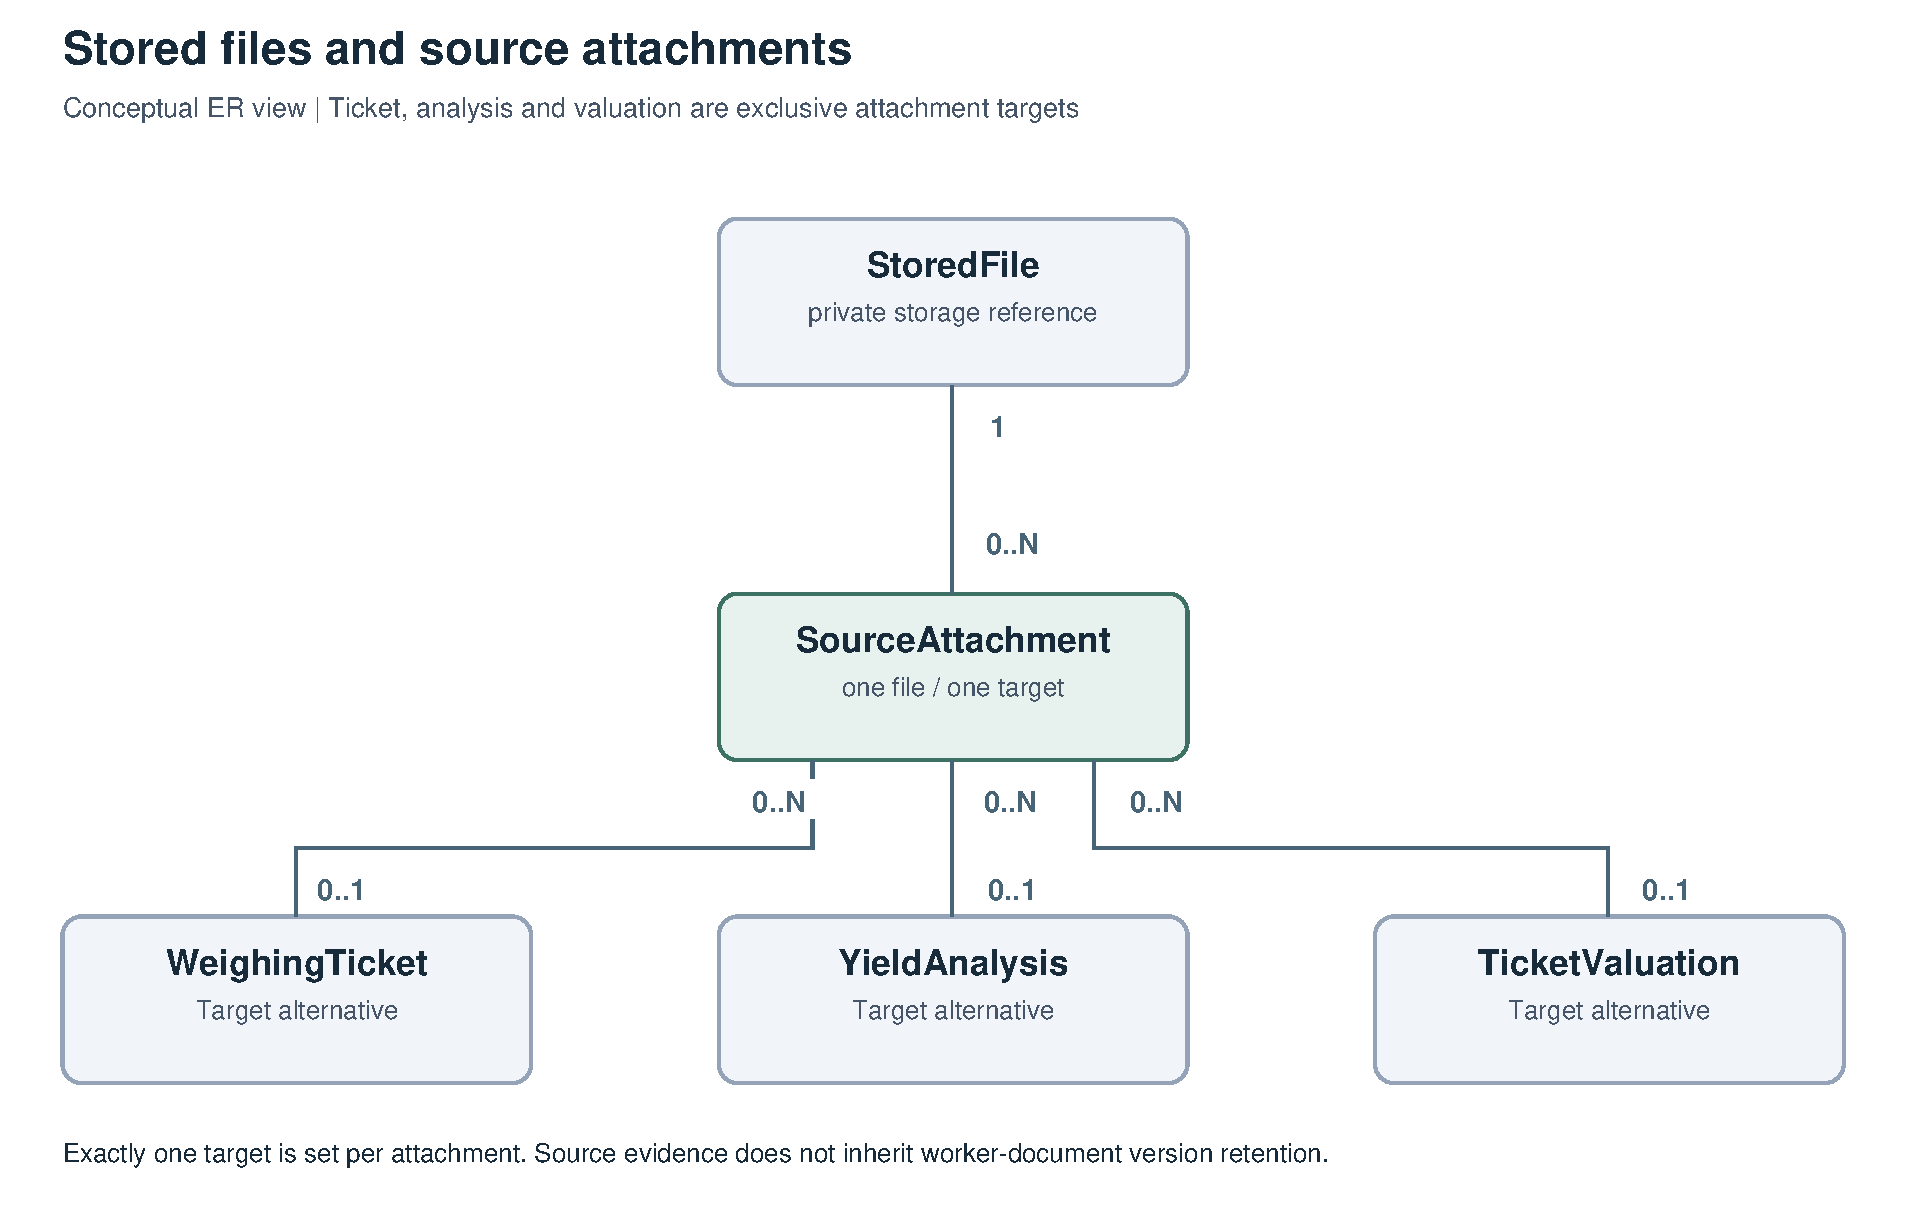
\includegraphics[width=\textwidth]{figures/er-source-files.pdf}
\caption{Source attachments and stored content. Each attachment targets exactly one source record; the three target links are exclusive alternatives.}
\label{fig:er-source-files}
\end{figure}

\FloatBarrier
\Needspace{10\baselineskip}
\subsection{Logical Data Model}
\label{sec:data-logical}
\paragraph{Conventions.}
Each table has a stable UUID id. Business-scoped tables carry workspace identity;
parent, worker, area and file references must stay in that workspace. Shared server
metadata comprises creation/update times, author where relevant and a revision
counter for concurrency, not a full field-change history. Accepted records satisfy
requiredness; a locally pending proposal is not central acceptance.
Optional parcel means whole-property scope; area uniqueness must handle NULL
explicitly. The table lists principal fields, not the full dictionary. Work timestamps are complete UTC instants with capture-time IANA timezone metadata. Device timezone drives entry/display; the initially device-suggested and owner-confirmed business timezone determines the shared start-based working date.
{\readabletable
\begin{longtable}{L{0.27}L{0.4}L{0.33}}
\caption{Principal entities, fields and relationships in the logical data model.}\label{tab:logical-model}\\
\toprule\rowcolor{TableHeader}
\textbf{Entity / table} & \textbf{Principal fields} & \textbf{Relationships / key} \\
\midrule\endfirsthead
\toprule\rowcolor{TableHeader}
\textbf{Entity / table} & \textbf{Principal fields} & \textbf{Relationships / key} \\
\midrule\endhead
\multicolumn{3}{r}{\footnotesize\itshape Continued on next page}\\\endfoot
\bottomrule\endlastfoot
User\newline \texttt{app\_\allowbreak{}user} & \mbox{\texttt{name}}, \mbox{\texttt{normalised\_email}}, \mbox{\texttt{account\_status}}, \mbox{\texttt{system\_role}}, \mbox{\texttt{provisioned\_by\_admin\_id}} & Global identity; unique normalised email. Verified changes preserve id. \\
\midrule
Workspace\newline \texttt{workspace} & \mbox{\texttt{name}}, \mbox{\texttt{business\_timezone}}, \mbox{\texttt{status}} & Single client workspace, pending until owner activation; timezone suggested from the creating device and explicitly confirmed; Owner through membership. \\
\midrule
WorkspaceMembership\newline \texttt{workspace\_\allowbreak{}membership} & \mbox{\texttt{user\_id}}, \mbox{\texttt{workspace\_role}}, \mbox{\texttt{access\_status}}, \mbox{\texttt{revoked\_at}} & User; unique workspace/User pair. \\
\midrule
ManagerInvitation\newline \texttt{manager\_\allowbreak{}invitation} & \mbox{\texttt{recipient\_email}}, \mbox{\texttt{invited\_by\_user\_id}}, \mbox{\texttt{invitation\_status}}, \mbox{\texttt{expires\_at}} & Intended verified recipient; issuer and accepted membership. \\
\midrule
AccessGrant\newline \texttt{access\_\allowbreak{}grant} & \mbox{\texttt{membership\_id}}, \mbox{\texttt{operation\_code}}, \mbox{\texttt{property\_id}} & Required property scope; parcels/current/future campaigns inherit it. Unique membership/operation/property; insurance constraint. \\
\midrule
WorkerAvailability\newline \texttt{worker\_\allowbreak{}availability} & \mbox{\texttt{membership\_id}}, \mbox{\texttt{worker\_id}} & Owner-explicit worker availability; unique membership/worker, same workspace; no other-property work authority. \\
\midrule
Property\newline \texttt{property} & \mbox{\texttt{name}}, \mbox{\texttt{textual\_location}}, \mbox{\texttt{declared\_area\_ha}}, \mbox{\texttt{olive\_varieties}} & Workspace; parent of Parcels. \\
\midrule
Parcel\newline \texttt{parcel} & \mbox{\texttt{property\_id}}, \mbox{\texttt{name}}, \mbox{\texttt{declared\_area\_ha}}, \mbox{\texttt{olive\_varieties}} & Property in the same workspace. \\
\midrule
HarvestCampaign\newline \texttt{harvest\_\allowbreak{}campaign} & \mbox{\texttt{name}}, \mbox{\texttt{planned\_start\_date}}, \mbox{\texttt{actual\_start\_date}}, \mbox{\texttt{actual\_end\_date}}, \mbox{\texttt{lifecycle\_status}} & Workspace; Planned/In progress/Closed; one or more coverage entries. \\
\midrule
CampaignCoverage\newline \texttt{campaign\_\allowbreak{}coverage} & \mbox{\texttt{campaign\_id}}, \mbox{\texttt{property\_id}}, \mbox{\texttt{parcel\_id}} & Campaign, Property, optional Parcel; unique selected area. \\
\midrule
Worker\newline \texttt{worker} & \mbox{\texttt{full\_name}}, \mbox{\texttt{telephone}}, \mbox{\texttt{official\_id\_type}}, \mbox{\texttt{official\_id\_country}}, \mbox{\texttt{official\_id\_number}}, \mbox{\texttt{can\_operate\_machinery}}, \mbox{\texttt{capability\_description}} & Workspace; no required User FK. \\
\midrule
WorkPlan\newline \texttt{work\_\allowbreak{}plan} & \mbox{\texttt{campaign\_id}}, \mbox{\texttt{work\_date}} & Campaign; unique campaign/date. \\
\midrule
PlannedAssignment\newline \texttt{planned\_\allowbreak{}assignment} & \mbox{\texttt{plan\_id}}, \mbox{\texttt{worker\_id}}, \mbox{\texttt{property\_id}}, \mbox{\texttt{parcel\_id}} & Plan, Worker, area; unique plan/worker/area. \\
\midrule
PlannedWorkPeriod\newline \texttt{planned\_\allowbreak{}work\_\allowbreak{}period} & \mbox{\texttt{assignment\_id}}, \mbox{\texttt{worker\_id}}, \mbox{\texttt{planned\_start}}, \mbox{\texttt{planned\_end}} & PlannedAssignment; checked worker reference. \\
\midrule
PlannedBreak\newline \texttt{planned\_\allowbreak{}break} & \mbox{\texttt{assignment\_id}}, \mbox{\texttt{break\_start}}, \mbox{\texttt{break\_end}}, \mbox{\texttt{counts\_as\_work}} & PlannedAssignment. \\
\midrule
DailyAttendance\newline \texttt{daily\_\allowbreak{}attendance} & \mbox{\texttt{worker\_id}}, \mbox{\texttt{work\_date}}, \mbox{\texttt{attendance\_status}} & Worker; unique workspace/worker/date. \\
\midrule
ActualWorkAssignment\newline \texttt{actual\_\allowbreak{}work\_\allowbreak{}assignment} & \mbox{\texttt{attendance\_id}}, \mbox{\texttt{worker\_id}}, \mbox{\texttt{campaign\_id}}, \mbox{\texttt{property\_id}} & Attendance, Campaign, area; optional source plan assignment. Unique attendance/campaign/area. \\
\midrule
WorkPeriod\newline \texttt{work\_\allowbreak{}period} & \mbox{\texttt{assignment\_id}}, \mbox{\texttt{worker\_id}}, \mbox{\texttt{actual\_start}}, \mbox{\texttt{actual\_end}}, \mbox{\texttt{task\_code}} & ActualWorkAssignment; the worker reference must match the associated actual assignment. \\
\midrule
WorkBreak\newline \texttt{work\_\allowbreak{}break} & \mbox{\texttt{attendance\_id}}, \mbox{\texttt{break\_start}}, \mbox{\texttt{break\_end}}, \mbox{\texttt{counts\_as\_work}} & DailyAttendance. \\
\midrule
Delivery\newline \texttt{delivery} & \mbox{\texttt{campaign\_id}}, \mbox{\texttt{destination\_name}}, \mbox{\texttt{delivery\_status}}, \mbox{\texttt{delivered\_at}}, \mbox{\texttt{cancellation\_reason}} & Campaign; one transport and one or more source batches; cancellation preserves dependants. \\
\midrule
TransportRecord\newline \texttt{transport\_\allowbreak{}record} & \mbox{\texttt{delivery\_id}}, \mbox{\texttt{driver\_worker\_id}}, \mbox{\texttt{vehicle\_reference}}, \mbox{\texttt{departure\_at}}, \mbox{\texttt{transport\_document\_reference}}, \mbox{\texttt{declared\_origin\_property\_id}}, \mbox{\texttt{declared\_origin\_parcel\_id}} & Unique Delivery; Worker driver. Declared origin is separate from OliveBatch. \\
\midrule
OliveBatch\newline \texttt{olive\_\allowbreak{}batch} & \mbox{\texttt{delivery\_id}}, \mbox{\texttt{property\_id}}, \mbox{\texttt{parcel\_id}}, \mbox{\texttt{collection\_origin}} & Delivery; source area within campaign coverage. \\
\midrule
WeighingTicket\newline \texttt{weighing\_\allowbreak{}ticket} & \mbox{\texttt{delivery\_id}}, \mbox{\texttt{assigned\_weight\_kg}}, \mbox{\texttt{reported\_weights}}, \mbox{\texttt{source\_metadata}}, \mbox{\texttt{source\_date}}, \mbox{\texttt{reported\_duration\_seconds}}, \mbox{\texttt{weighing\_started\_at}}, \mbox{\texttt{weighing\_ended\_at}}, \mbox{\texttt{excess\_time\_value}}, \mbox{\texttt{excess\_time\_unit}} & Unique delivery; canonical reported accepted assigned kg plus optional source timing. \\
\midrule
TicketAdjustment\newline \texttt{ticket\_\allowbreak{}adjustment} & \mbox{\texttt{ticket\_id}}, \mbox{\texttt{adjustment\_type}}, \mbox{\texttt{reported\_value}}, \mbox{\texttt{unit}} & WeighingTicket. \\
\midrule
YieldAnalysis\newline \texttt{yield\_\allowbreak{}analysis} & \mbox{\texttt{delivery\_id}}, \mbox{\texttt{yield\_percentage}}, \mbox{\texttt{analysis\_date}} & Unique delivery. Weight through that delivery's ticket; no copied reference weight. \\
\midrule
TicketValuation\newline \texttt{ticket\_\allowbreak{}valuation} & \mbox{\texttt{ticket\_id}}, \mbox{\texttt{amount}}, \mbox{\texttt{currency}}, \mbox{\texttt{valuation\_status}} & Unique WeighingTicket; current value only. \\
\midrule
Document\newline \texttt{document} & \mbox{\texttt{title}}, \mbox{\texttt{document\_category}}, \mbox{\texttt{form\_type}}, \mbox{\texttt{worker\_id}} & One required Worker; one current accepted source, without consultable history. \\
\midrule
DocumentVersion\newline \texttt{document\_\allowbreak{}version} & \mbox{\texttt{document\_id}}, \mbox{\texttt{version\_number}}, \mbox{\texttt{source\_file\_id}}, \mbox{\texttt{origin\_kind}}, \mbox{\texttt{template\_id}}, \mbox{\texttt{template\_revision}}, \mbox{\texttt{is\_withdrawn}} & Unique document reference: one current accepted source. New identity/sequence on replacement; superseded source, signature and PDF deleted. \\
\midrule
WorkerSignature\newline \texttt{worker\_\allowbreak{}signature} & \mbox{\texttt{worker\_id}}, \mbox{\texttt{version\_id}}, \mbox{\texttt{initiated\_by\_user\_id}}, \mbox{\texttt{client\_signed\_at}}, \mbox{\texttt{form\_response}} & Worker, Version, User, StoredFile; unique worker/version; worker must equal Document.worker\_id. \\
\midrule
StoredFile\newline \texttt{stored\_\allowbreak{}file} & \mbox{\texttt{storage\_key}}, \mbox{\texttt{original\_filename}}, \mbox{\texttt{media\_type}}, \mbox{\texttt{byte\_size}} & Private content; unique storage key. \\
\midrule
SourceAttachment\newline \texttt{source\_\allowbreak{}attachment} & \mbox{\texttt{stored\_file\_id}}, \mbox{\texttt{ticket\_id}}, \mbox{\texttt{analysis\_id}}, \mbox{\texttt{valuation\_id}} & StoredFile; exactly one populated target FK. \\
\midrule
DocumentTemplate\newline \texttt{document\_\allowbreak{}template} & \mbox{\texttt{name}}, \mbox{\texttt{document\_category}}, \mbox{\texttt{template\_file\_id}}, \mbox{\texttt{revision}}, \mbox{\texttt{field\_schema}} & Workspace; template StoredFile and reviewed field schema. \\
\midrule
DocumentRendition\newline \texttt{document\_\allowbreak{}rendition} & \mbox{\texttt{version\_id}}, \mbox{\texttt{worker\_id}}, \mbox{\texttt{stored\_file\_id}}, \mbox{\texttt{generated\_at}} & Unique version/worker; derived PDF StoredFile; associated accepted signature; worker matches Document. \\
\end{longtable}}

Other ticket weights and template/invitation/input schemas use validated JSON;
core relationships remain foreign keys. Assigned kg is a canonical typed ticket column populated from KILOS ASIGNADOS, not duplicated in JSON or analysis. A monetary penalty is a reported
TicketAdjustment with EUR unit and known application status. Unique delivery
references enforce one ticket and one analysis even under concurrent requests.
The selected Spanish template/revision and input snapshot freeze the current generated source context;
the rendition never replaces that source. Repeated rendering does not create
another worker/version signature.

\Needspace{9\baselineskip}
\subsection{Data Dictionary}
\label{sec:data-dictionary}
The complete current field inventory is maintained separately in
\nolinkurl{technical/data-architecture/data-dictionary.tex}. The following meanings
are essential to interpreting the condensed model.
{\readabletable
\begin{longtable}{L{0.31}L{0.69}}
\caption{Key field groups and their meanings.}\label{tab:data-dictionary-summary}\\
\toprule\rowcolor{TableHeader}
\textbf{Field group} & \textbf{Meaning} \\
\midrule\endfirsthead
\toprule\rowcolor{TableHeader}
\textbf{Field group} & \textbf{Meaning} \\
\midrule\endhead
\multicolumn{2}{r}{\footnotesize\itshape Continued on next page}\\\endfoot
\bottomrule\endlastfoot
Identity and scope & User identifies an account; Worker identifies a person within a business, using a separate UUID. Required worker fields: full name, telephone and official identification type/country/number. Workspace references and composite keys prevent cross-business links. \\
\midrule
Dates and timezone & Confirmed business timezone governs daily grouping; device timezone drives entry/display with preserved capture context. Full instants preserve overnight and clock-change meaning. Enter minutes; report hours/minutes. Entry, event and acceptance times differ. Only selected/expected workers await attendance; complete confirmed periods require a task. \\
\midrule
Delivery state & In transport, delivered or cancelled. Campaign lifecycle is separately Planned, In progress or Closed. Cancellation has reason/actor/time, preserves source records and excludes their contributions. \\
\midrule
Reported weights & assigned\_weight\_kg is the ticket's canonical cooperative-reported accepted assigned kg. Other weights preserve meanings/units. Unknown is NULL, not zero. \\
\midrule
Yield reference & yield\_percentage is the reported result. Its weighted-average reference is read through the delivery ticket, not stored again on the analysis. \\
\midrule
Weighing and penalties & Start/end and excess duration/unit reproduce the ticket. Monetary penalties are reported adjustments; no scale-rate calculation or second deduction follows. \\
\midrule
Load provenance & OliveBatch stores actual origins and known quantities separately from declared transport origin. It has no source monetary amounts; mixed-load money remains unallocated by area. No proportional or dominant-parcel allocation is inferred. \\
\midrule
Version protection & Keep only the current document source until successful replacement, then delete the old source, signature and PDF for every category. No consultable history; pending old-source signing is ineligible and follows \identifier{Q-DOC-04} recovery. \\
\midrule
Generation and renditions & Template/revision and reviewed input snapshot identify generated sources. A rendition is a worker-specific derived signed PDF linked to its source version. \\
\midrule
Financial/local state & Reported provisional/final status is distinct from pending/accepted synchronisation. Offline financial content requires financial authorisation. \\
\midrule
Files & PDF/JPG/PNG uploads have the 10~MB limit. Availability/upload state does not prove server acceptance of dependent records. \\
\end{longtable}}

\paragraph{Source integrity.}
An accepted document source has a protected \texttt{content\_hash} under \identifier{SEC-08};
the full dictionary records the conditional requiredness by file purpose. This is
integrity metadata, not signer authentication or a replacement for version identity.

\paragraph{Operational source fields.}
The full reference records client-confirmed total/assigned-weight semantics, accepted percentage and independently printed duration.
Document subtype identifies the form; reviewed inputs are version snapshots. A
required acceptance/refusal choice is bound to signature evidence and rendered in
the appropriate form area. Signed, server-accepted and consent accepted are separate.

\paragraph{Technical account authority.}
User.system\_role distinguishes standard users from the Technical Administrator;
provisioned\_by\_admin\_id records the initial owner's issuer. It does not grant
access to agricultural records/files. Workspace and initial owner membership
remain pending until recipient activation; the complete field reference specifies
these additions within the existing 33-entity model.

\subsection{Integrity Constraints}
\label{sec:data-integrity}
Identity and row-level checks are insufficient for cross-record invariants. Enforce
the following at central transactional acceptance, including concurrent requests.
{\readabletable
\begin{longtable}{L{0.24}L{0.59}L{0.17}}
\caption{Cross-record integrity constraints.}\label{tab:integrity-constraints}\\
\toprule\rowcolor{TableHeader}
\textbf{Scope} & \textbf{Essential constraint} & \textbf{Rules} \\
\midrule\endfirsthead
\toprule\rowcolor{TableHeader}
\textbf{Scope} & \textbf{Essential constraint} & \textbf{Rules} \\
\midrule\endhead
\multicolumn{3}{r}{\footnotesize\itshape Continued on next page}\\\endfoot
\bottomrule\endlastfoot
Ownership/access & One owner per active workspace; all business parent/file links in scope. Apply owner-reviewed grants and mandatory insurance access. & \identifier{BR-001}--BR-004 \\
\midrule
Coverage/work & Parcel belongs to property; assignments fit coverage. Preserve unique attendance and non-overlapping same-worker planned/actual intervals, checked separately. Reopening precedes confirmed changes where required. & \identifier{BR-005}--BR-021 \\
\midrule
Delivery/results & Accepted delivery has transport and source batch(es). Unique delivery FK on ticket and analysis. Analysis weighting reads the same delivery ticket. Cancelled parents accept no new source results. & \identifier{BR-031}--BR-033 \\
\midrule
Corrections and cancellation & Validate affected campaign scopes, chronology, coverage and dependent data; no cascade deletion. Cancellation preserves sources and removes contributions. Hard deletion requires no dependent tickets, analyses, valuations or evidence; remove composed
transport/batch rows together. & \identifier{BR-031}, \identifier{BR-038} \\
\midrule
Values/evidence & One current valuation per ticket. Exactly one target per source attachment; combine all applicable association and complete-file consultation permissions, without mandatory monetary-content classification or automatic redaction. & \identifier{BR-024}, \identifier{BR-034}--BR-036 \\
\midrule
Versions/signatures & Unique document/version sequence and accepted worker/version signature. Signer must equal the document's single Worker reference. One current accepted source per document. Successful replacement deletes the old source, signature and PDF, even when signed; invalidate old-source signing without transferring or recreating it. Temporary local proposal recovery follows \identifier{Q-DOC-04}, not a version-history policy. & \identifier{BR-023}--BR-030 \\
\midrule
Generation/rendition & Generated source has reviewed template/revision/input snapshot; accepted rendition uses associated worker/version signature and same-workspace files. Source identity remains immutable. & \identifier{BR-041} \\
\midrule
Files/acceptance & Apply upload format/limit checks. No current source before file readiness. Revision/idempotency checks prevent duplicate effects; cleanup respects all retained references. & \identifier{BR-021}, \identifier{BR-044} \\
\end{longtable}}

Coverage reservation, intervals, sequence allocation and minimum-child counts need
transactional enforcement. File cleanup is recoverable across database/object-store
boundaries. The team verifies replacement file cleanup, positive/non-overlapping break validation, out-of-period warnings and recovery mechanisms against the approved NFRs.


Planned campaigns may overlap. Serialise competing Planned-to-In-progress starts,
Closed-to-In-progress reopens and execution coverage changes over every relevant
property/parcel key, including whole-property versus child conflicts. Actual-date
checks remain independent of planned dates and archival. Two accepted competing
executions must not result from concurrent offline requests.

Worker name, telephone and official type/country/number are required before accepting
a new worker. The internal UUID is the primary key; same-business duplicate matches
produce review, not an automatic merge or mandatory unique-document rejection.
Accept worker identity before dependent work or driving. Document creation
requires that accepted worker online; signing requires the accepted individual source. Every confirmed complete WorkPeriod has its actual task.
Do not create unresolved attendance alerts for unrelated unselected workers.

For accepted document sources, enforce the immutable file reference/digest required
by \identifier{SEC-08}. Integrity metadata is protected with the associated source; a digest does
not establish the worker's identity or make a drawn mark a certified signature.

\paragraph{Source examples.}
Validate ticket metadata against its schema; preserve literal identifiers and
separate total kg, canonical accepted assigned kg and accepted percentage. Printed duration may differ from
elapsed timestamps and requires an interpretation note; valid chronology still
applies. MEDIANERIA never automatically populates yield or deductions. A new
application signature for a decision-bearing form requires an explicit valid choice,
immutably bound to worker/version evidence and rendered identically on its PDF.
External signed uploads may have unknown structured response. Every uploaded/generated Document has exactly one worker, fixed after acceptance;
check that the signature and rendition worker matches the version parent.

\paragraph{Technical administration and single-client setup.}
Enforce administrator authority centrally for owner provisioning and enforce a
single deployment workspace/initial owner, including concurrent requests. Pending
workspace and owner membership activate atomically after recipient verification.
Only deployment bootstrap assigns the administrator role; normal owner/manager
requests cannot elevate it. Membership-scoped business APIs/files require their
own grants, even for an authenticated administrator. Invited manager creation
requires the valid owner-issued recipient context. Activation challenges remain
protected technical records, separate from the 33 domain entities.

\subsection{Data Lifecycle and History}
\label{sec:data-lifecycle}
Archival/inactivation preserves record identities; campaign archival is independent
of closure. Delivery cancellation stores its reason and preserves linked results,
while excluding their contributions. Interrupted/refused trips use cancellation;
a new attempt creates a new delivery/transport. Ordinary corrections retain current
values rather than permanent field-change history.

\identifier{BR-026} defines current-only document retention for every category.
Keep the source and its signature/PDF until a complete replacement is accepted;
then delete the superseded source, signature and derived PDF, without inherited
signing or consultable history. Failed uploads preserve the current graph. An
explicit source-attachment replacement similarly switches the file only after
readiness and deletes the former file. Generated inputs remain frozen while their
source exists, rather than changing with profiles or templates.

Deletion reaches prepared copies through Section~\ref{sec:offline-sync}. Ineligible
old-source signing is rejected and needs fresh worker review/signing of a current
source; temporary protected recovery/outcome information is not a version-history
store. Minimal deletion/idempotency metadata prevents replay from recreating files.
Central backup expiry and restore suppression follow \identifier{REL-04}; deletion
is not represented as immediate removal from every disconnected device or backup.

Privacy requests use the manual procedure in \identifier{PRV-04}: the owner receives
and follows the request and a designated technical responsible person intervenes
when authorised. Business closure and ownership transfer remain excluded. Hosting,
named operational ownership and processing notices/bases still require deployment
preparation; the chosen replacement policy is not a claim of legal certification.
Security events retain their separate minimal 90-day schedule, not file contents
or ordinary business correction history.

\subsection{Local and Central Data}
\label{sec:data-local-central}
The central database holds accepted records; private object storage holds accepted
files. IndexedDB is selected to store account/workspace-isolated prepared subsets and
durable proposals. Synchronisation follows Section~\ref{sec:offline-sync}.
{\readabletable
\begin{longtable}{L{0.25}L{0.43}L{0.32}}
\caption{Local preparation and central storage responsibilities.}\label{tab:local-central}\\
\toprule\rowcolor{TableHeader}
\textbf{Data group} & \textbf{Prepared / pending locally} & \textbf{Central responsibility} \\
\midrule\endfirsthead
\toprule\rowcolor{TableHeader}
\textbf{Data group} & \textbf{Prepared / pending locally} & \textbf{Central responsibility} \\
\midrule\endhead
\multicolumn{3}{r}{\footnotesize\itshape Continued on next page}\\\endfoot
\bottomrule\endlastfoot
Reference/plans & Assigned properties, coverage, workers and prepared plans; supported planning proposals. & Authoritative identity, grants, availability, campaign state and plan acceptance. Structure and existing-profile administration remain online; explicit starts and basic worker creation have pending dependencies. \\
\midrule
Attendance/work & Prepared attendance, assignments, intervals/breaks and authorised correction proposals. & Unique daily state, intervals, dates, scopes, revision/conflict validation. \\
\midrule
Documents/signing & Current prepared insurance and explicitly selected current sources for signing; pending drawings and worker-specific renditions. & Version/file readiness, signer eligibility, evidence, current-only replacement deletion and accepted rendition; old-source signing is invalidated. Source generation remains online. \\
\midrule
Deliveries/results & Prepared deliveries, tickets/accepted assigned kg, analyses and supported entry/correction/cancellation proposals; separate attachment status. & Single ticket/analysis constraints, provenance, cancellation/dependency validation and source files. \\
\midrule
Financial information & Permitted prepared values, penalties, financial/mixed files and consultation/entry/correction proposals. & Financial authorisation, current valuation and accepted source amounts. No unrestricted preparation or automatic redaction. \\
\midrule
Indicators/PDF & Available baseline plus identifiable proposals; local arrival may enable provisional results. Financial results require grants. Record scope, freshness, exclusions and pending status. & Server-accepted arrivals and source values; only Delivered, non-cancelled parents contribute under \identifier{BR-038}. \\
\end{longtable}}

Operation envelopes, revisions, change cursors, deletion markers and dependency
ordering follow Section~\ref{sec:offline-sync}. The local store retains complete
pending worker identification and stable UUID references across attendance, work
and driving. Accept parent identities and campaign starts before dependants,
preserving proposals needing resolution. Document source acceptance is online;
only accepted individual sources may be prepared for offline signing.

Local loss may destroy proposals never received centrally. Offline access follows
\hyperref[br:002]{\identifier{BR-002}}; local-only/cloud-only selectable modes are outside scope.
Routine interaction follows Section~\ref{sec:offline-interaction}.

\subsection{Physical Data Model}
\label{sec:data-physical}
PostgreSQL is the selected central relational store; exact DDL, indexes and
transactional enforcement still require implementation and verification.
{\readabletable
\begin{longtable}{L{0.28}L{0.72}}
\caption{Proposed physical data representations.}\label{tab:physical-model}\\
\toprule\rowcolor{TableHeader}
\textbf{Family} & \textbf{Proposed representation} \\
\midrule\endfirsthead
\toprule\rowcolor{TableHeader}
\textbf{Family} & \textbf{Proposed representation} \\
\midrule\endhead
\multicolumn{2}{r}{\footnotesize\itshape Continued on next page}\\\endfoot
\bottomrule\endlastfoot
Identity/scope & UUID primary and operation ids; composite scope keys support same-workspace references. Integer revision counters support concurrency. \\
\midrule
Time & Full event/signing/acceptance instants use timestamptz; date for work/campaign/expiry dates. Workspace business\_timezone stores a validated timezone identifier. This type preserves the instant but not the original timezone/offset, so preserve capture-time IANA timezone metadata separately. Device timezone governs entry/display; the confirmed business timezone governs shared working-date assignment and filters. Minute-level input does not reduce timestamps to time-of-day values. \\
\midrule
Quantities/money & numeric for accepted assigned kg, other weights, areas, yield and amounts. Monetary amounts use two decimal places; weights/areas preserve source precision and calculations retain full stored values. The team verifies database precision and range constraints. \\
\midrule
Source/configuration & Schema-validated jsonb for other reported weights, invitation configuration, template fields and reviewed generation inputs. Core associations remain FKs. \\
\midrule
Files & Private object storage for source, template, signature and rendition bytes; StoredFile metadata and server-side format/size/access validation. Upload limit: 10~MB = 10,000,000 bytes; JPEG/JPG share the same accepted image format. \\
\end{longtable}}

The instant/timezone distinction follows the
\href{https://www.postgresql.org/docs/18/datatype-datetime.html\#DATATYPE-DATETIME-INPUT-TIMESTAMPS}{PostgreSQL date/time documentation}.

\paragraph{Essential keys and indexes.}
Use unique membership, coverage/assignment, attendance, plan, current-document-source,
worker/version signature and ticket-valuation keys. Unique delivery references
enforce one ticket/analysis; a unique version/worker key identifies a rendition.
Index campaign/area/date queries, worker intervals, document worker/version links and
attachment targets. Owner and whole-property/parcel uniqueness need explicit
partial/NULL handling; minimum-child counts and dependency checks are transactional.

Enforce planned and actual same-worker overlaps separately through exclusion or
equivalent serialised validation. Serialise execution reservations across a property
and its parcels, including start/reopening and coverage changes. Unlocked
read-then-insert checks or ordinary indexes alone are insufficient.

Store required official identification as text, preserving leading zeroes; use a
non-unique workspace/\allowbreak{}type/\allowbreak{}country/\allowbreak{}normalised-number lookup index. Worker and
operation UUIDs support client creation. Campaign lifecycle values are
\texttt{planned}, \texttt{in\_progress} and \texttt{closed}.

The physical design also requires an operation-outcome ledger, authorised
change/deletion feed and protected owner-review recovery store. Preserve template
snapshots and retained signed/cancelled-record references. Local prepared subsets,
outbox and file metadata need not mirror every central table. Local authorisation
metadata stores online-validation and expiry instants; its approved policies and
unresolved implementation mechanisms follow Sections~\ref{sec:business-rules}--\ref{sec:solution-architecture}.

\identifier{SEC-08} requires an integrity digest for each accepted document source, stored with
protected metadata and verified before association. Keep client confirmation and server acceptance timestamps distinct. A unique document reference permits one current accepted DocumentVersion; replacement creates its new identity and removes old signing/rendition rows and file references consistently. Salted password hashes, session/token
verifiers, security-event logs,
deletion/restriction recovery metadata and deployment key controls are technical
persistence concerns, not additional business actors/entities. Their implementation
and approved technical retention limits follow Section~\ref{sec:non-functional-requirements}
and Section~\ref{sec:nfr-targets}.

AccessGrant has required property scope and a unique membership/operation/property
key; there is no independent campaign/parcel scope discriminator. WorkerAvailability
uses same-workspace membership/worker FKs and a unique pair. Validate invitation
scope at creation and acceptance, including revoked/archived property context.
Security events use a 90-day server-event policy; minimal operation outcomes and
change/deletion markers use their separate 90-day policies. Store originator and
accepting owner separately for reviewed recovery. These mechanisms do not add
ordinary field-change history or override the current-only document replacement policy.

\paragraph{Provisioning fields.}
Add checked system role and nullable self-referencing administrator issuer on
\texttt{app\_user}. Existing normal users migrate to standard authority; never infer
administrator status from an Owner membership. Use a deployment-level single-client
transactional guard and pending-to-active workspace/membership checks. A protected
bootstrap procedure prepares the initial administrator; normal APIs never expose
administrator self-registration. Token verifiers and password hashes remain
technical authentication persistence. No additional domain entity is needed.

